\documentclass[a4paper]{article}

%% Language and font encodings
\usepackage[english]{babel}
\usepackage[utf8x]{inputenc}
\usepackage[T1]{fontenc}

%% Sets page size and margins
\usepackage[a4paper,top=3cm,bottom=2cm,left=3cm,right=3cm,marginparwidth=1.75cm]{geometry}

%% Useful packages
\usepackage{amsmath}
\usepackage[table,xcdraw]{xcolor}
\usepackage{tabularx,booktabs}
\usepackage{graphicx}
\usepackage[colorinlistoftodos]{todonotes}
\usepackage[colorlinks=true, allcolors=blue]{hyperref}
\usepackage{amsmath}
\usepackage{tikz}
\usepackage{tkz-tab}
\usepackage{caption}
\usepackage{latexsym}
\usepackage{amssymb}
\usepackage{amsmath}
\usepackage{subcaption}
\usepackage{mathtools}
\usepackage{multirow}
\usepackage{listings}
\usepackage{color}
\usepackage{epsfig}
\usepackage{epstopdf}
\usepackage{soul}

%% Useful packages
\usepackage[table,xcdraw]{xcolor}
\usepackage{tabularx,booktabs}
\newcolumntype{C}{>{\centering\arraybackslash}X} % centered version of "X" type
\newcolumntype{b}{X}
\newcolumntype{s}{>{\hsize=.5\hsize}X}
\newcolumntype{v}{>{\hsize=.3\hsize}X}

\definecolor{mygreen}{rgb}{0,0.6,0}
\definecolor{mygray}{rgb}{0.5,0.5,0.5}
\definecolor{mymauve}{rgb}{0.58,0,0.82}


\lstdefinestyle{customc}{
  belowcaptionskip=1\baselineskip,
  breaklines=true,
  frame=L,
  xleftmargin=\parindent,
  language=C,
  showstringspaces=false,
  basicstyle=\footnotesize\ttfamily,
  keywordstyle=\bfseries\color{green!40!black},
  commentstyle=\itshape\color{purple!40!black},
  identifierstyle=\color{blue},
  stringstyle=\color{orange},
}

\lstdefinestyle{customasm}{
  belowcaptionskip=1\baselineskip,
  frame=L,
  xleftmargin=\parindent,
  language=[x86masm]Assembler,
  basicstyle=\footnotesize\ttfamily,
  commentstyle=\itshape\color{purple!40!black},
}

\lstset{escapechar=@,style=customc}

\usetikzlibrary{automata,arrows,positioning,calc}
\usetikzlibrary{shapes,snakes}

% Commands for commenting in inside the text content
\newcommand{\sergio}[1]{\textcolor{brown}{#1}}
\newcommand{\sergiost}[1]{\textcolor{brown}{\st{#1}}}
\newcommand{\franky}[1]{\textcolor{red}{#1}}


%%% TITLE
\title{Komondor: an Event-Based Wireless Network Simulator for Next-Generation IEEE 802.11ax WLANs}
\author{Sergio Barrachina-Mu\~noz and Francesc Wilhelmi}

\begin{document}
\maketitle

\begin{abstract}
Komondor is a wireless network simulator that includes novel mechanisms for next-generation WLANs, such as Dynamic Channel Bonding or enhanced Spatial Reuse. One of Komondor's main purposes is to emulate the behavior of IEEE 802.11ax-2019 networks, which main challenge is spectral efficiency in dense deployments. Furthermore, due to the growing popularity of autonomous systems and the tendency of WLANs to use learning, Komondor is intended to include intelligent agents that make decisions that allow enhancing the network performance. 

In this document we provide an overview of the Komondor simulator, making insight on its main features, its operational mode and its development stages. This document is therefore aimed at providing to potential contributors the necessary information for getting into Komondor, so that its operational mode can be properly understood and the code can be modified/complemented. Komondor has been conceived as an open source tool that contributes to the ongoing research in wireless networks. For that, all the contents are published at the following public repository: \url{https://github.com/wn-upf/Komondor}. Any interested researcher is invited to collaborate.

\end{abstract}

\tableofcontents

\listoffigures

\listoftables

\newpage

%%%%%%%%%%%%%%%
% INTRODUCTION
%%%%%%%%%%%%%%%
\section{Introduction}
\label{section:introduction}

Komondor \cite{barrachina2017komondor} is an event-based simulator based on COST \cite{chen2002reusing}, a CompC++ library that allows generating discrete event simulations.\footnote{COST main website: \url{http://www.ita.cs.rpi.edu/cost.html}} Komondor is mostly intended to reproduce the novel techniques included in the IEEE 802.11ax-2019 amendment \cite{tgax2017draft}, which is called to become a benchmark in next-generation wireless networks. Furthermore, due to the increasing popularity of learning-based approaches in WLANs, our simulator is being built to allow the inclusion of intelligent agents that make decisions in simulation time. The decision of building a new wireless networks simulator is based on $i)$ the lack of 11ax-oriented simulators that include novel techniques, $ii)$ the need of generating a tool able to simulate intelligent agents behavior and, $iii)$ the difficulty in extending other existing solutions (e.g., ns-3) towards our abovementioned main goals. 
	
Komondor is a long-term and iterative project which goals are mostly focuses in providing a reliable and accurate IEEE 802.11ax simulator. In this document we present its version v1.0, which includes the core functionalities to provide a basic operation.
	
In this document we describe the main features of the Komondor simulator and system model considerations, both from theoretical and development perspectives. The main contributions done in this document are listed below:
\begin{itemize}
	\item We provide an overview of the first version of the Komondor simulator.
	\item We describe the implementation done for each of the included functionalities, as well as the main considerations done.
	\item We provide a set of validations that ensure the proper operation of the presented simulator.
	\item We provide implementation details in case the reader is interested in extending and/or deeply understanding the simulator.
\end{itemize}	
	
%%%%%%%%%%%%%%%
% PROJECT OVERVIEW
%%%%%%%%%%%%%%%
\section{Project Overview}
\label{section:project_overview}

Komondor is composed by several modules that allow performing simulations with a high degree of freedom. Here we provide some details on the most important modules, as well as on their practical execution. Figure \ref{fig:komondor_flowchart} summarizes the modules that constitute Komondor. A set of inputs (nodes information, simulation time, etc.) are provided to the main module (\texttt{komondor.cc}), which is in charge of initializing and monitoring the simulation. Once nodes are initiated, the core of the simulation takes place, where packet exchanges are held based on the provided wireless design (further detailed in Section \ref{section:system_model}). Finally, when the simulation runs out, a set of outputs are generated in order to shed some light on the network performance.
\begin{figure}[h!]
	\centering
	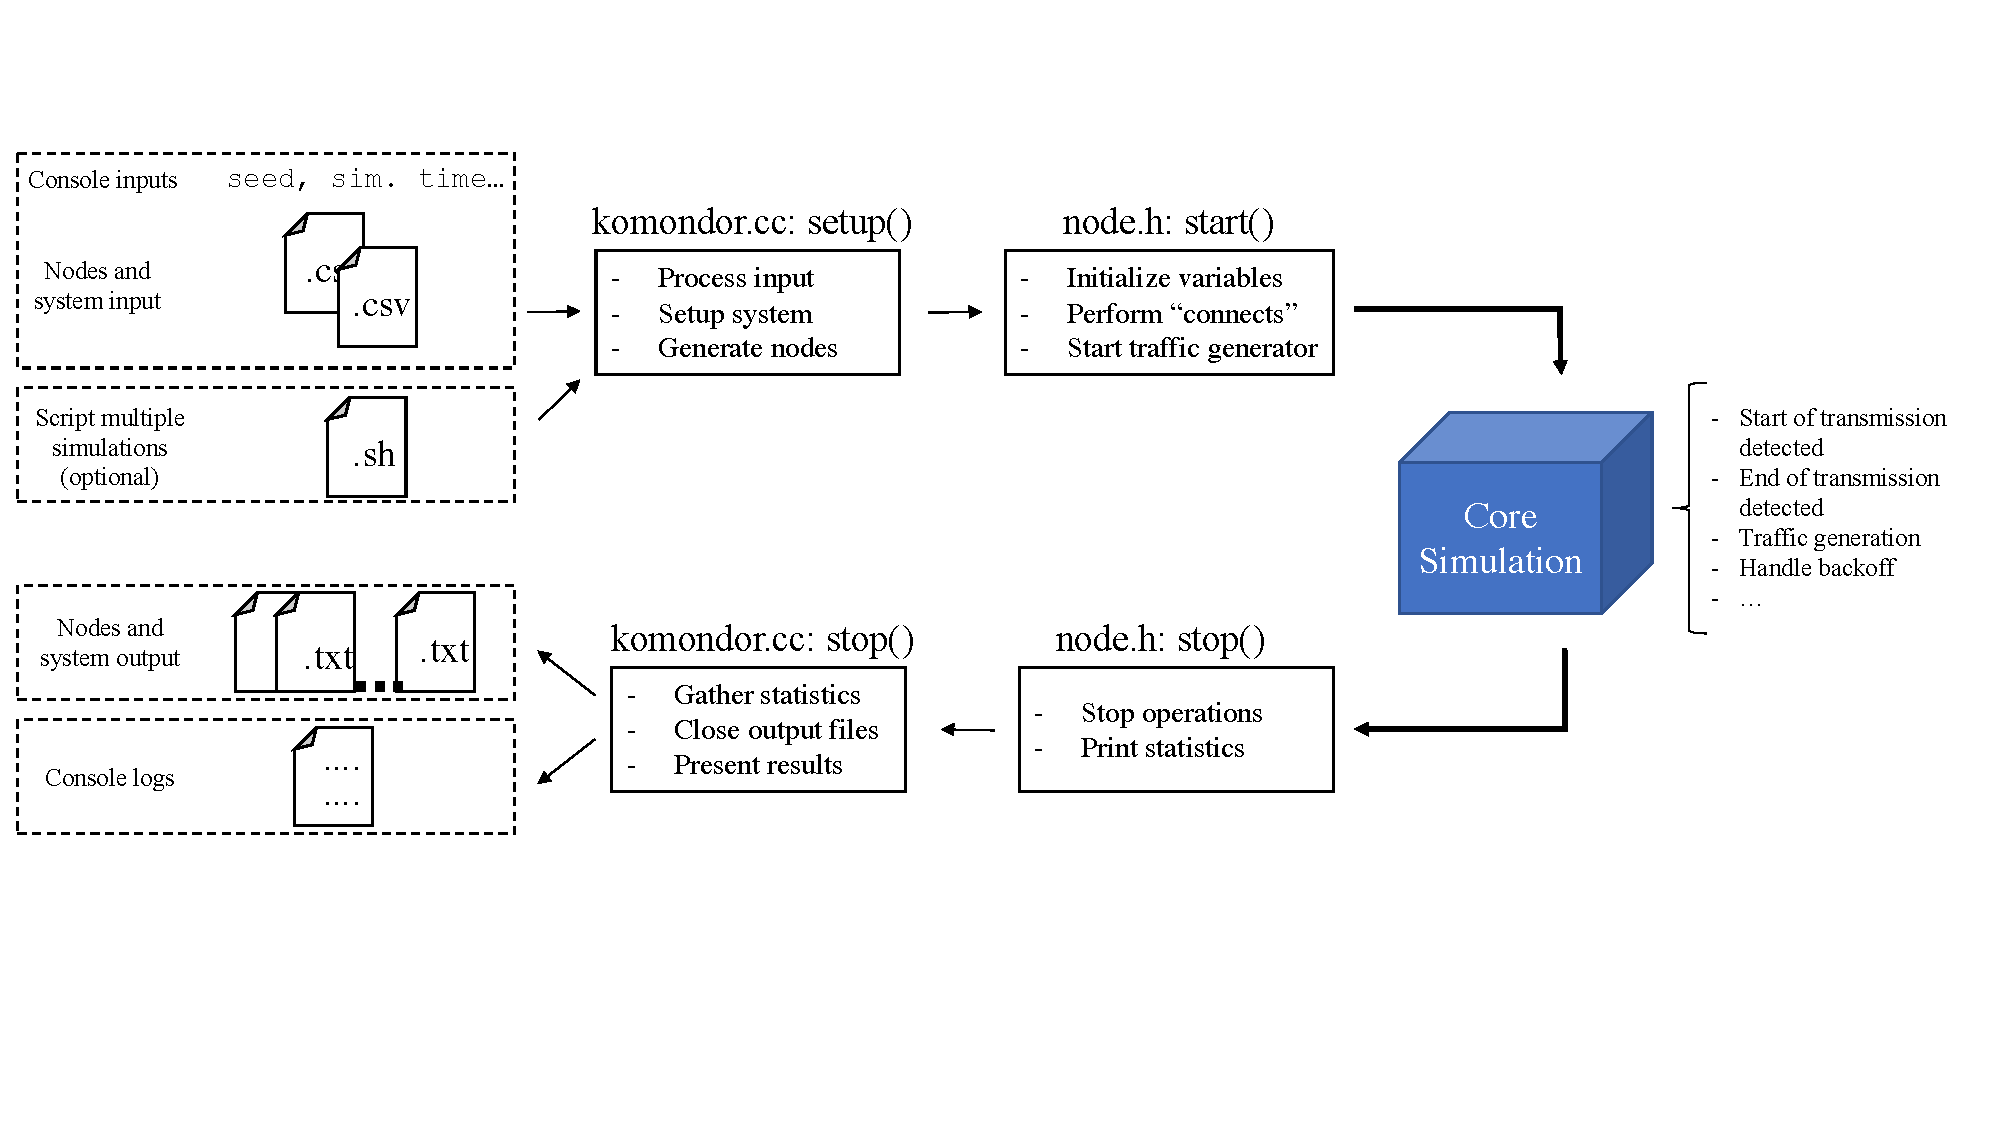
\epsfig{file=images/komondor_flowchart, width=15cm}
	\caption{Komondor flowchart}
	\label{fig:komondor_flowchart}
\end{figure}		

% COST 
\subsection{COST}
\label{section:cost}

In order to provide a deep understanding of Komondor from a developer standpoint, it is important to first comprehend the COST library, which allows building interactions between components (e.g., wireless nodes). Such interaction is achieved through synchronous and asynchronous events. While the former are messages explicitly exchanged between components through input/output ports, the later are based on timers. 

In practice, components perform a set of operations until a significant event occurs. For instance, a node that is decreasing its backoff (i.e., current operation) may freeze it when an overlapping node occupies the channel (i.e., an event). Moreover, the node may start a transmission when the backoff timer is over (i.e., a trigger). Figure \ref{fig:cost} shows the schematic of a COST component, which is characterized by its inports and outports, and a set of timers. 
\begin{figure}[h!]
	\centering
	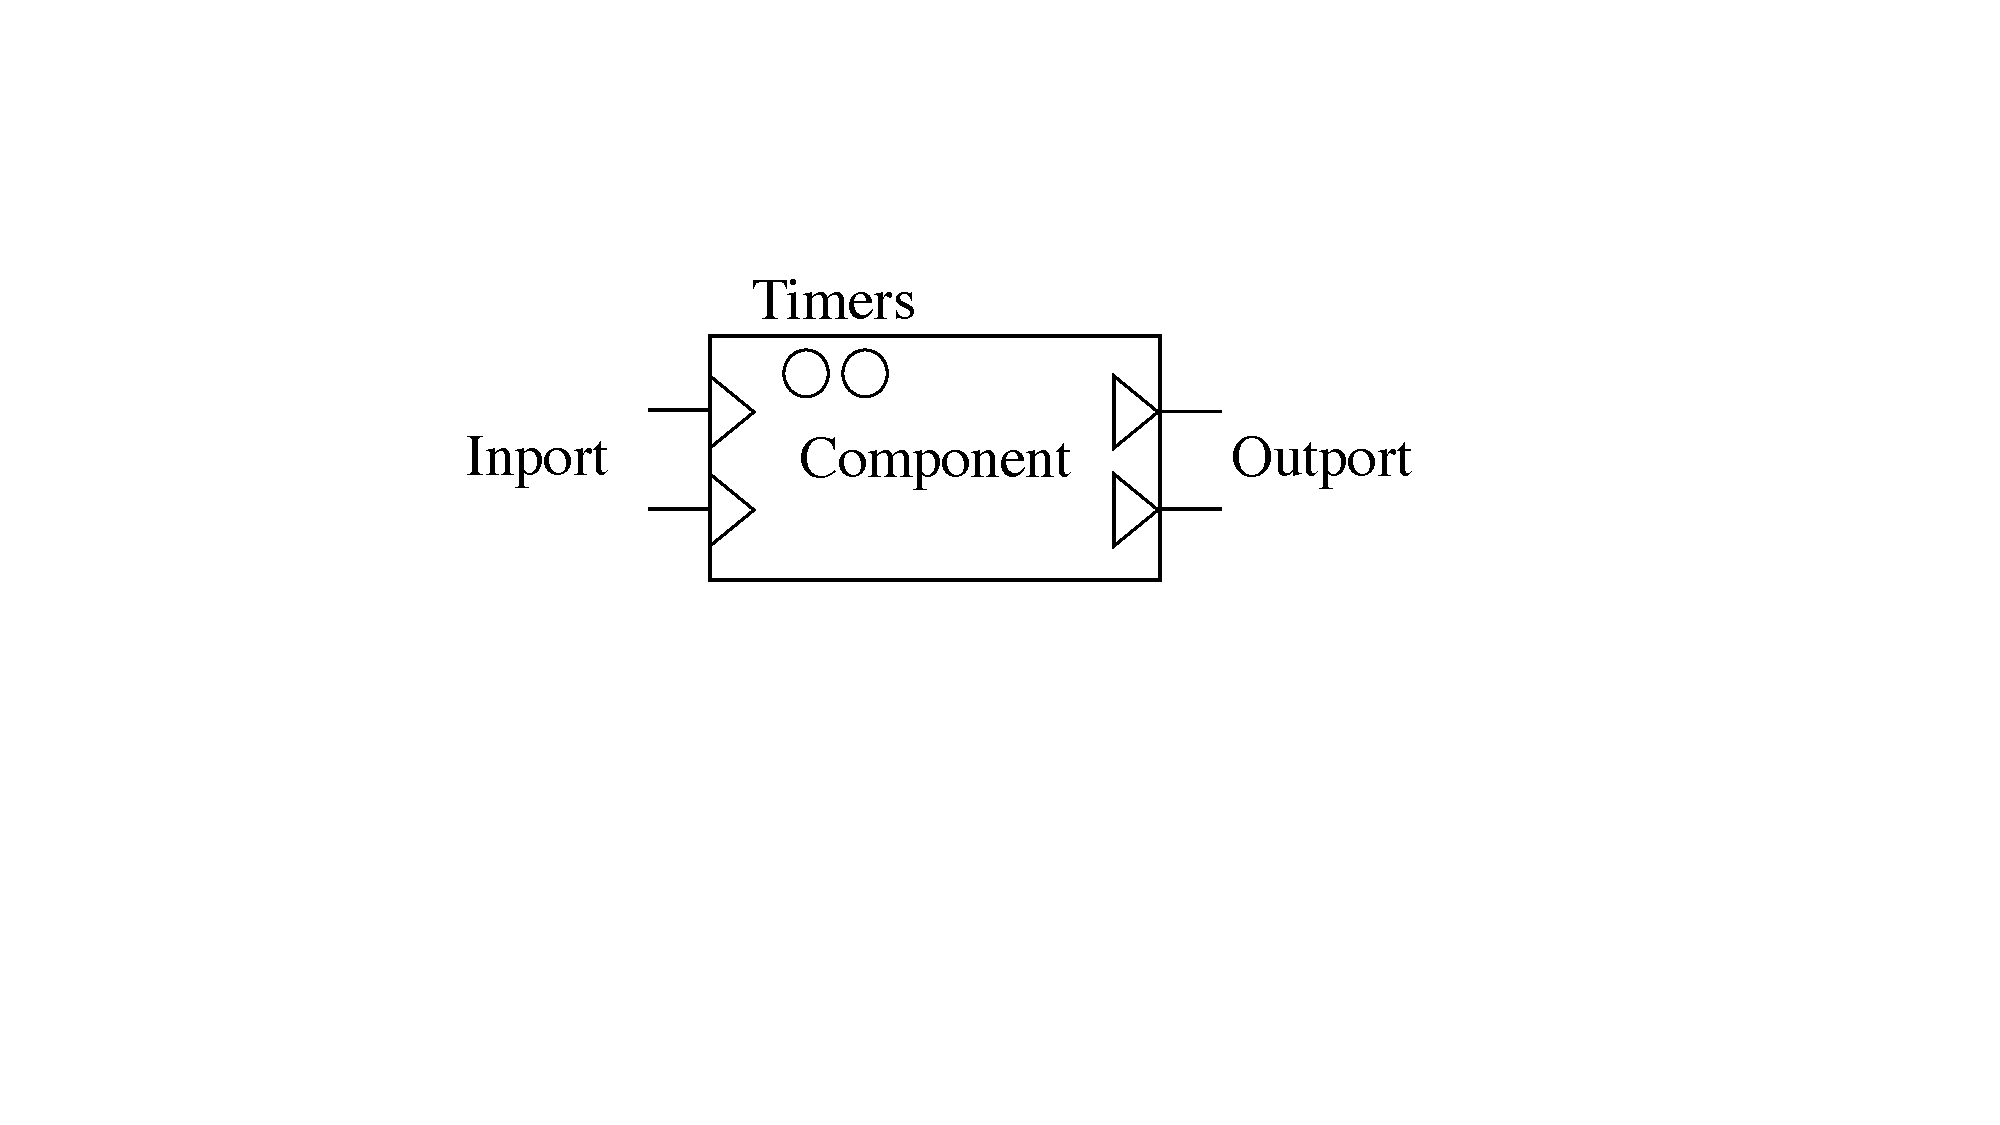
\epsfig{file=images/cost.pdf, width=7cm}
	\caption{COST component. While inports and outports allow to directly communicate with other components, timers trigger events specific to the component.}
	\label{fig:cost}
\end{figure}	

% Project organization
\subsection{Files Organization}
\label{section:files}		
To properly understand the Komondor's operation, it is important to know how the project allocated in \href{https://github.com/wn-upf/Komondor}{Github} is organized. In particular, the project is divided into three main folders: \textit{Apps}, \textit{Code} and \textit{Documentation}. \textit{Apps} and \textit{Documentation} folders are intended to contain additional material that supplements the core Komondor's infrastructure (this document, for instance, is inside the \textit{Documentation} folder). Here we focus on the code part, which is organized as follows (refer to Figure \ref{fig:komondor_files} as well):
\begin{itemize}
	\item \textbf{COST}: constitute the Komondor's primitive operation. Here we find the CompC++ library that allows generating discrete event simulations. For further information about COST, please refer to its main \href{http://www.ita.cs.rpi.edu/cost.html}{website}. 
	\item \textbf{main}: contains the core files (\texttt{komondor\_main.cc}, \texttt{node.h}, \texttt{agent.h} and \texttt{central\_controller.h}) that are in charge of orchestrating all the simulation.  \texttt{komondor\_main.cc} is the main component, which initializes all the other components of \textit{Type II}. All these modules are aware of the existence of the simulation time. In addition to the core components, here we find \texttt{build\_local}, a bash script that compiles the libraries for executing the code. Note that file \texttt{compcxx\_komondor\_main.h} is also required to carry out such a compilation.
	\item \textbf{methods}: by following clean architecture guidelines, independent methods used by core files are contained in the methods folder. Several libraries are provided according to the nature of their functions. For instance, \texttt{backoff\_methods.h} contains methods to handle the backoff operation in DCF.
	\item \textbf{structures}: the Komondor simulator considers several header files to carry out its operation. Among them, we find \texttt{wlan.h}, which defines the main characteristics of a WLAN (WLAN id, list of associated STAs, etc.). In addition, the \texttt{notification.h} structure allows to define the information to be exchanged between devices. 
	\item \textbf{learning\_modules}: here we find the implementation of Machine Learning (ML) methods that receive feedback about the networks performance in simulation time. 
	\item \textbf{list\_of\_macros.h}: all the static parameters (e.g., constants) are contained in this file.
	\item \textbf{input}: contains the input files that allow building the simulation environment.
	\item \textbf{output}: contains the data generated by Komondor as a result of a given simulation.	
	\item \textbf{scripts\_multiple\_executions}: contains bash scripts to perform multiple simulations.
\end{itemize} 

\begin{figure}[h!]
	\centering
	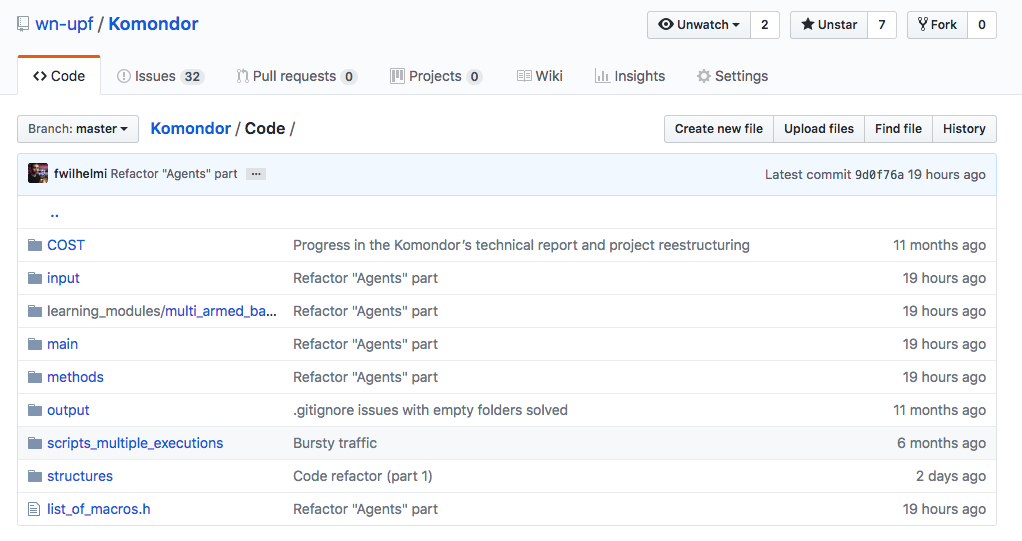
\epsfig{file=images/komondor_files, width=12cm}
	\caption{Komondor files organization}
	\label{fig:komondor_files}
\end{figure}	

%%%  Komondor main features
\subsection{Komondor Main Features}
\label{section:features}
Komondor aims to realistically capture the operation of wireless networks. Henceforth, it reproduces actual transmissions on a per-packet basis. For that, nodes properties (e.g., location, transmit power, CCA threshold) are taken into account during data exchange procedures. The initial version of the Komondor simulator includes the following functionalities:
\begin{itemize}
	\item \textbf{Flexible input files processing with error control}: network capabilities can be introduced into the simulator in a very flexible manner. Moreover, an input checker is provided in order to identify the most prominent errors in the input provided by the user.
	\item \textbf{IEEE 802.11ax WLANs features implemented in version v1.0}:
	\begin{itemize}
		\item \textbf{Distributed Coordination Function (DCF)}: the Carrier Sense Multiple Access with Collision Avoidance (CSMA/CA) captures the basic Wi-Fi operation for accessing the channel. Moreover, Contention Window (CW) adaptation is considered.
		\item \textbf{Channel Bonding (CB)}: several channel ranges can be selected during transmissions in order to maximize the spectrum efficiency.
		\item \textbf{Packet aggregation}: several MPDUs can be aggregated into the same PPDU in order to reduce the generated communication overheads.
		\item\textbf{ Dynamic Modulation Coding Scheme (MCS)}: the MCS is negotiated between any transmitter-receiver pair according to the Signal-to-Interference-and-Noise Ratio (SINR).
		\item \textbf{Ready-to-Send/Clear-to-Send (RTS/CTS) and Network Allocation Vector (NAV)}: nodes exchange packets before transmitting in order to allocate the channel and prevent collisions.
	\end{itemize}
	\item \textbf{Statistics}: different metrics of interest are gathered and properly presented.
\end{itemize}

Future development stages are considered to include other features such as OFDMA, MU-MIMO transmissions, beamforming, or dynamic transmit power and CST adjustment.
	
%%%%%%%%%%%%%%%
% DESIGN PRINCIPLES
%%%%%%%%%%%%%%%
\section{Komondor Design Principles}
\label{section:system_model}
In this Section we describe the Komondor design principles, which lay the foundations of the simulator. In particular, we define the main entities involved in the simulation, and the states-based design that rule the operation of nodes.

\subsection{Main entities}
\label{section:main_entities}
As roughly defined in Section \ref{section:project_overview}, the Komondor simulator is orchestrated by the \texttt{komondor\_main.cc} class, which can be found at the \textit{/Komondor/Code/main} folder. First of all, it initializes all the entities involved in the simulation (nodes, agents, etc.) according to the input provided by the user. Then, when the simulation ends, the \texttt{komondor\_main.cc} class collects all the necessary information, displays it and concludes the execution.

Regarding the entities involved in the simulation itself, we currently find the following classes (also located in the \textit{/Komondor/Code/main}):
\begin{itemize}
	\item \texttt{node.h}: it defines the operation of a wireless node, which can be either of type AP or STA. Differentiating between these two types of nodes has important implications and, until this version, AP is the only type of node that can initiate data transmissions. The core operation followed by a node entity is further detailed in Section \ref{section:core_operation}.
	\item \texttt{agent.h}: the agent entity can be optionally enabled for a given WLAN. In practice, an agent may decide the configuration of the WLAN to which it is associated. Further details about the implementation of agents are provided in Section \ref{section:agents}.
	\item \texttt{central\_controller.h}: this entity is responsible of collecting all the information generated by nodes and/or agents, and to provide a centralized operation to indicate certain configuration parameters. To this date, the central controller is only logically implemented, and no centralized mechanisms are provided to modify the configuration of its attached WLANs.
\end{itemize}

\subsection{States-based operation}
\label{section:states}
To understand the implementation provided by Komondor to simulate the IEEE 802.11 operation, it is important to show the states that are contemplated for the \texttt{node.h} class. Figure \ref{fig:state_diagram} illustrates all the possible states and the interactions between them.

\begin{figure}[h]
	\centering
	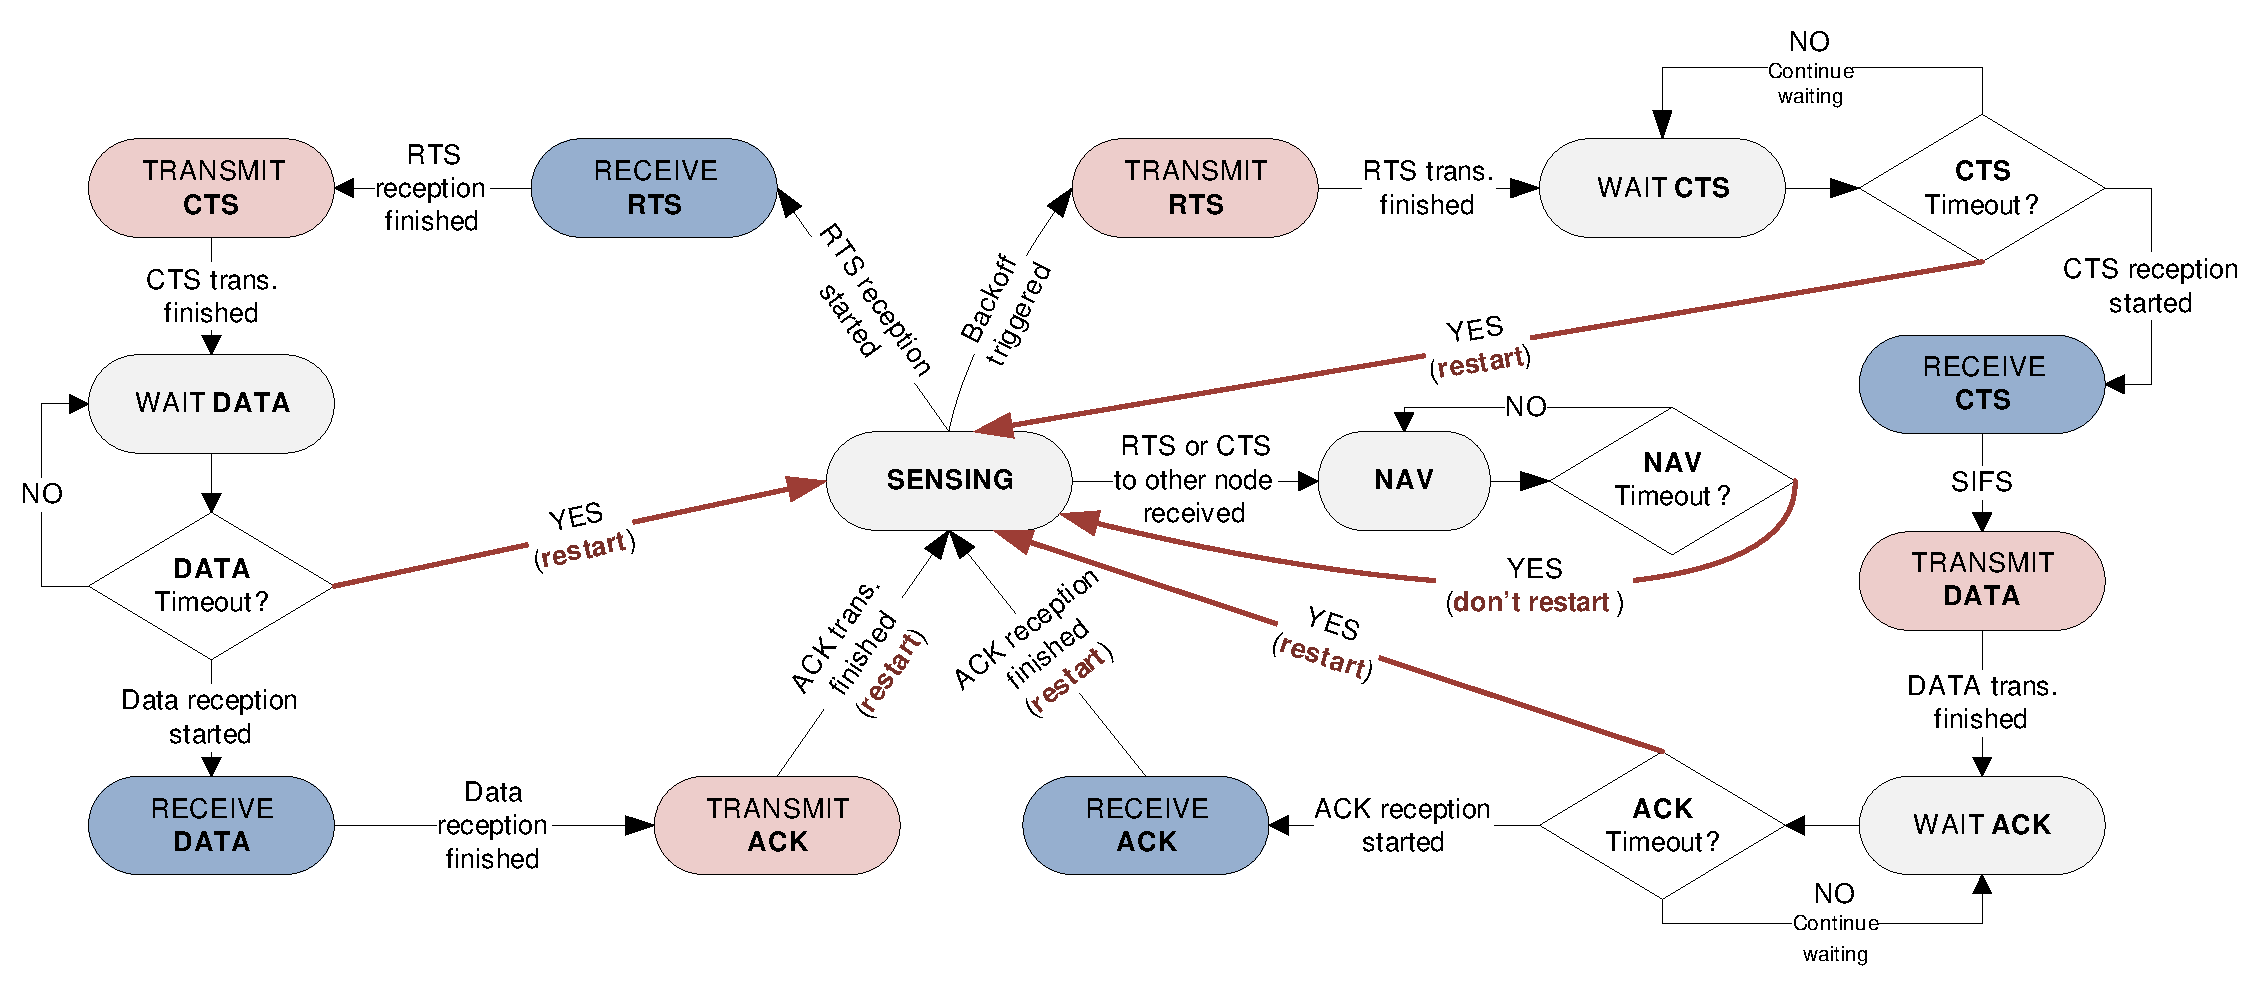
\includegraphics[width=\textwidth]{images/state_diagram.eps}
	\caption{States diagram for Komondor nodes.}    
	\label{fig:state_diagram}
\end{figure}

A given node starts the simulation in the \texttt{SENSING} state, and transits to other states according to the subsequent events. For instance, a transmitter finishing its backoff would transit to \texttt{TRANSMIT RTS}, provided that the channel is clear and the transmission can be initiated. Accordingly, the node receiving the RTS frame would transit from \texttt{SENSING} to \texttt{RECEIVE RTS}. Moreover, nodes in the carrier sense area of such a transmission are expected to go to \texttt{NAV} state. It is important to remark that the RTS/CTS operation is mandatory for this version of Komondor, since it is part of the core design. Implementing optional RTS/CTS is part of the future work.

The states-oriented design that is shown in Figure \ref{fig:state_diagram} is very useful to have control on the different simulation phases and to define accurate output logs. . It is particularly necessary to provide the timeouts of the different transmitted frames, and to determine the behavior to be followed by a node for a given situation. For instance, the \texttt{restart} operation varies according to the origin state. If the \texttt{restart} is called from \texttt{RECEIVE ACK}, then the data transmission can be determined as successful. Otherwise, if the origin state is, for instance, \texttt{WAIT DATA}, then we can ensure that the transmission failed.

%%%%%%%%%%%%%%%
% DESIGN PRINCIPLES
%%%%%%%%%%%%%%%
\section{Komondor's IEEE 802.11 Core Operation}
\label{section:core_operation}
The core operation of Komondor is described in this Section, thus providing an overview of the most important mechanisms that allow simulating the IEEE 802.11 operation. Note that the contents described in this Section compose the core of the simulator which, from a contributor's point of view, cannot be modified without affecting to the proper system's operation (validated in \textcolor{red}{[CITE HERE THE VALIDATIONS PAPER]}). In particular, we provide the implementation details at PHY,  MAC and upper communication layers.

%%% PHY foundations
\subsection{PHY}
\label{section:phy}
Here we describe the implementation of the PHY layer and the main assumptions that have been considered.
	
	% Signal transmission
	\subsubsection{Channel representation and signal transmission}	
	Komondor, unlike other network simulators, does not consider an environment-related entity (i.e., the frequency band) with which nodes interact. In contrast, every node maintains its own representation of the channel, according to what they sensed from their physical location. Such a representation is updated each time a new interaction with the channel occurs (i.e., when a node enters or leaves the channel). At the code level, nodes are connected through a set of inports/outports, which allow updating the variables maintained for channel representation. Specifically, there are two methods in the \texttt{node.h} class that handle interactions with the channel, which are called \texttt{InportSomeNodeStartTX} and \texttt{InportSomeNodeFinishTX}. The former is activated when a node starts a transmission, and the latter when is leaves the channel. From the transmitter's point of view, the abovementioned methods are activated at all the other nodes when using \texttt{outportSelfStartTX} and \texttt{outportSelfFinishTX}, respectively. As shown later in Section \ref{section:mac}, these outports are ruled by the channel access management methods.
	
	For any transmission, the signal received at all the other nodes depends on the channel effects and propagation losses (further defined in Section \ref{section:propagation}). It is important to note that the same power will be sensed at a given receiver along the entire frame transmission. Such an assumption is reasonable if we consider that frame transmissions typically last a very short time.
	
	% Interference management
	\subsubsection{Interference management and packet losses}
	\label{section:interference}
	As previously defined, nodes maintain their own channel representation, which is updated each time a third party starts/finishes a packet transmission. In particular, at any time, each node knows the additive interference generated by all the nodes that are currently transmitting. Such an information allows to manage the channel access and to determine whether an incoming transmission can be properly decoded or not. 
	
	The method that updates the information of every frequency channel available to the WLAN (note that adjacent channel interference can be also considered) is \texttt{UpdateChannelsPower()}. This method is called each time there is a change in the environment, i.e., when either \texttt{InportSomeNodeStartTX} or \texttt{InportSomeNodeFinishTX} are triggered by their respective outports. Then, according to the node's current state, different actions are performed. For instance, in state \texttt{SENSING}, a node noticing a new transmission is expected to check whether its backoff countdown can continue or not. Moreover, in case of being in any \texttt{RECEIVING} state, the node would check if the currently received frame is lost due to the new generated interference. Related to this, another important assumption is that the Signal to Interference and Noise Ratio (SINR) of every packet transmission must be kept above a capture effect (CE) threshold, which is an input parameter. Otherwise, the packet is lost. Specifically, a \emph{stronger-first} interference pattern is considered, so that any frame is properly decoded only if posterior transmissions do not generate high enough interference to discard it. Note that a dominant data transmission is not going be considered at a given receiver that is already receiving any type of data from another node. In such case, both transmissions are considered to be lost. The stronger-first CE principle is shown in Figure \ref{fig:capture_effect}. 
	\begin{figure}[h]
		\centering
		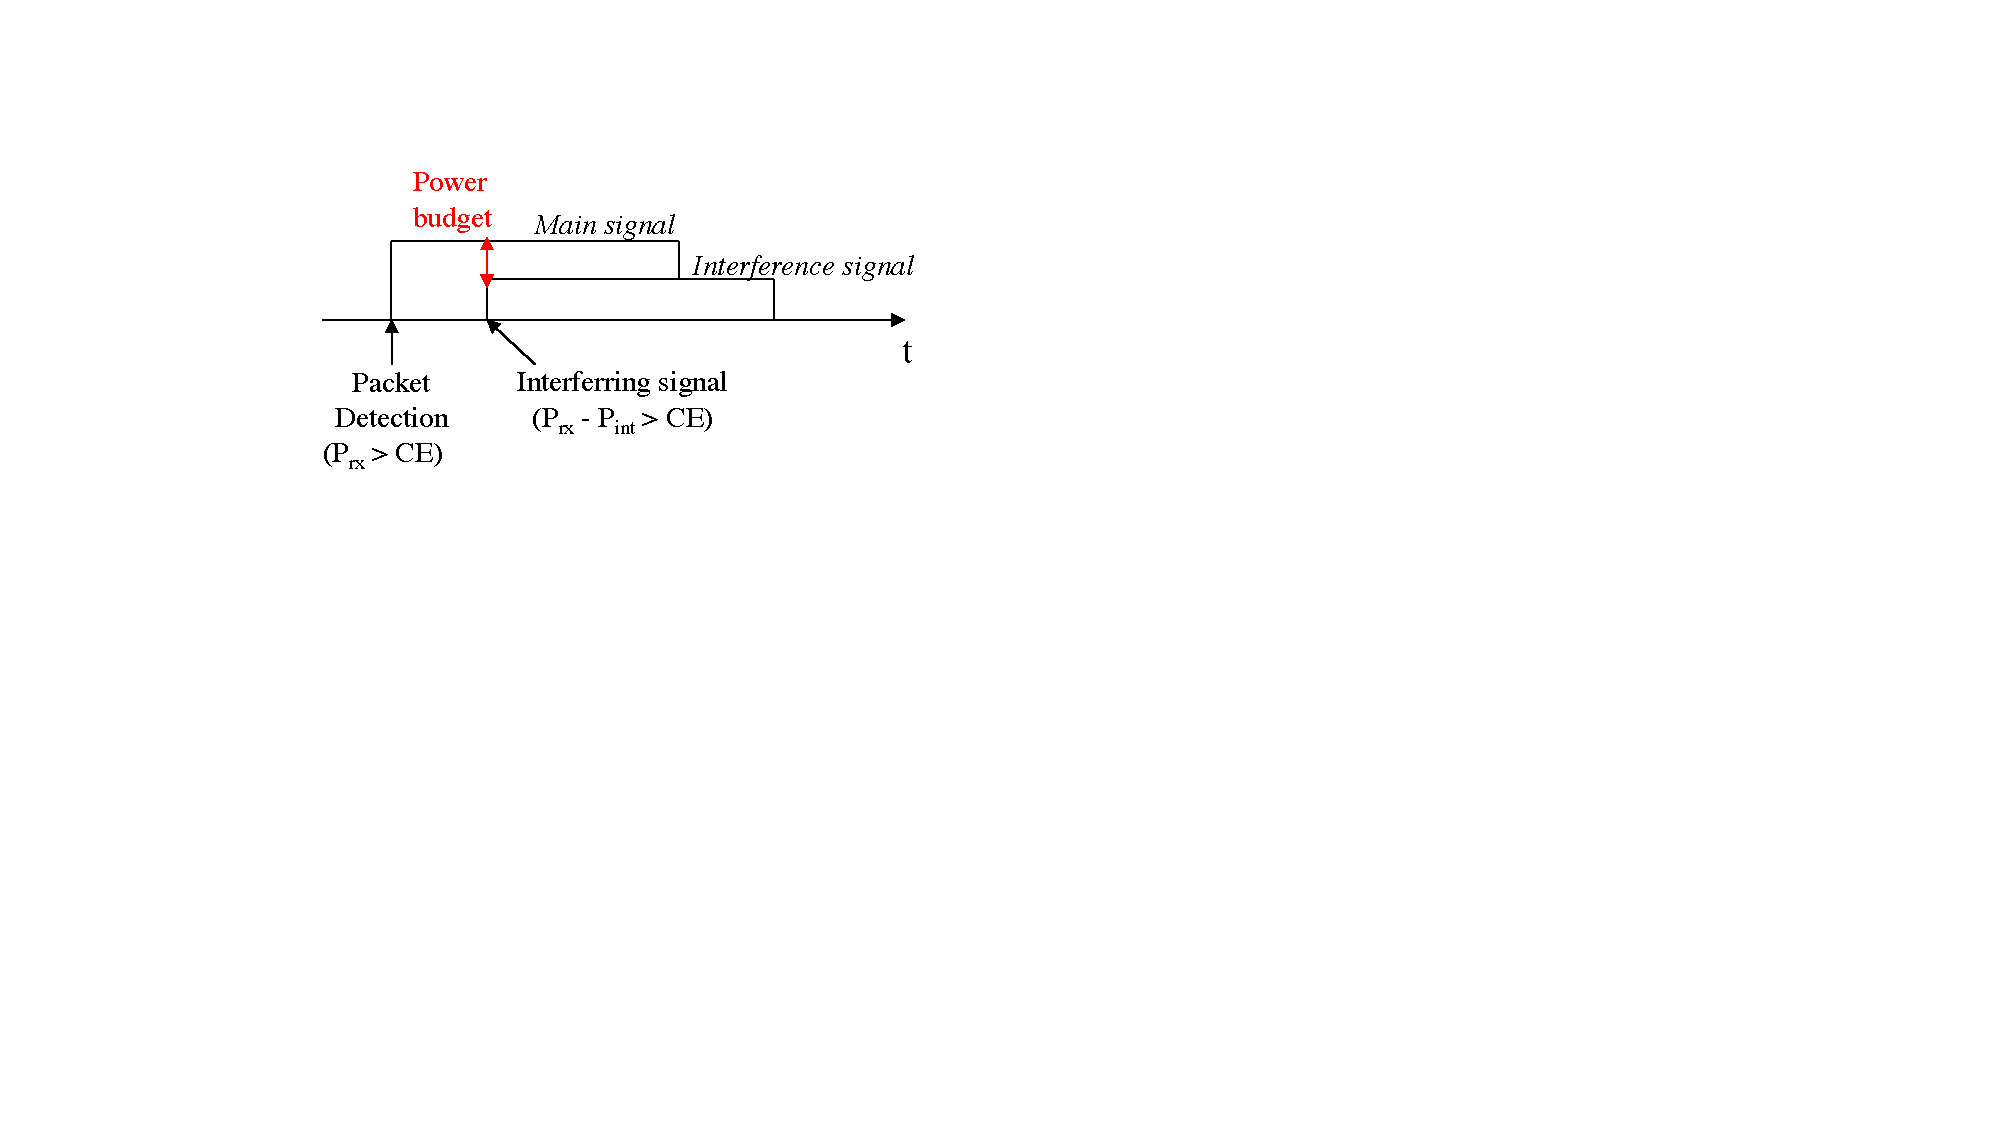
\includegraphics[width=0.6\textwidth]{images/capture_effect.pdf}
		\caption{Capture effect condition for a frame transmission.}    
		\label{fig:capture_effect}
	\end{figure}
	
	The CE condition is one of the reasons why packet losses may occur. In particular, Komondor contemplates several types of packet losses, which are informed to the transmitter in simulation time. The idea is to provide detailed ``off-line'' information about the interactions between nodes, so that packet losses can be properly understood when the simulation finishes. Note that such an information is not used in any different way than for generating statistics. The type of packet losses handled by Komondor are listed in Table \ref{tbl:packet_losses}.
	\begin{table}[]
		\centering
		\begin{scriptsize}
		\begin{tabular}{|l|l|}
			\hline
			\multicolumn{1}{|c|}{\textbf{Packet loss type}} & \multicolumn{1}{c|}{\textbf{Description}}                                                                                                                                             \\ \hline
			PACKET\_LOST\_DESTINATION\_TX                   & The destination is already transmitting any frame                                                                                                                                     \\ \hline
			PACKET\_LOST\_LOW\_SIGNAL                       & \begin{tabular}[c]{@{}l@{}}The signal strength of the attempted transmission \\ is not strong enough to be decoded, i.e., it is lower \\ than the receiver's sensitivity\end{tabular} \\ \hline
			PACKET\_LOST\_INTERFERENCE                      & \begin{tabular}[c]{@{}l@{}}The sensed interference is greater than the\\  receiver's sensitivity\end{tabular}                                                                         \\ \hline
			PACKET\_LOST\_PURE\_COLLISION                   & \begin{tabular}[c]{@{}l@{}}Two or more nodes transmit to the same destination \\ and their signal strengths are enough to be decoded\end{tabular}                                     \\ \hline
			PACKET\_LOST\_LOW\_SIGNAL\_AND\_RX              & \begin{tabular}[c]{@{}l@{}}The destination is any receiving state and the attempted \\ transmission's signal strength is not strong enough to be \\ decoded\end{tabular}              \\ \hline
			PACKET\_LOST\_SINR\_PROB                        & \begin{tabular}[c]{@{}l@{}}The packet lost due to SINR probability, which is \\ associated to the Modulation and Coding Scheme \\ (MCS) used\end{tabular}                             \\ \hline
			PACKET\_ACK\_LOST                               & Specific for ACK losses                                                                                                                                                               \\ \hline
			PACKET\_LOST\_RX\_IN\_NAV                       & \begin{tabular}[c]{@{}l@{}}The intended receiver is in virtual carrier sensing \\ (state \textbackslash{}texttt\{NAV\})\end{tabular}                                                  \\ \hline
			PACKET\_LOST\_BO\_COLLISION                     & \begin{tabular}[c]{@{}l@{}}Two nodes transmit simultaneously because they chose \\ the same backoff value\end{tabular}                                                                \\ \hline
			PACKET\_LOST\_OUTSIDE\_CH\_RANGE                & \begin{tabular}[c]{@{}l@{}}The frame is transmitted outside the primary channel \\ of the receiver\end{tabular}                                                                       \\ \hline
			PACKET\_LOST\_CAPTURE\_EFFECT                   & The CE condition is not accomplished at the receiver                                                                                                                                  \\ \hline
		\end{tabular}
	\end{scriptsize}
	\caption{Types of packet losses handled by Komondor.}
	\label{tbl:packet_losses}
	\end{table}
		
%%% MAC foundations
\subsection{MAC}
\label{section:mac}
Once the PHY layer has been presented, now we introduce the operation carried out at the MAC, which mostly refers to channel access and frames formatting.

	% Channel Access
	\subsubsection{Channel access}
	In Komondor, the channel access is ruled by the Distributed Coordination Function (DCF), which combines Carrier Sense Multiple Access with Collision Avoidance (CSMA/CA) with Binary Exponential Backoff (BEB). Accordingly, transmissions are carried out if the target channel (or set of channels) has been empty for a given Backoff (BO) time, which is computed according to a dynamic Contention Window (CW). The PHY implementation allows the MAC layer to perform the channel access procedures. Figure \ref{fig:dcf_operation} shows an example of the DCF operation. 
	\begin{figure}[h!]
		\centering
		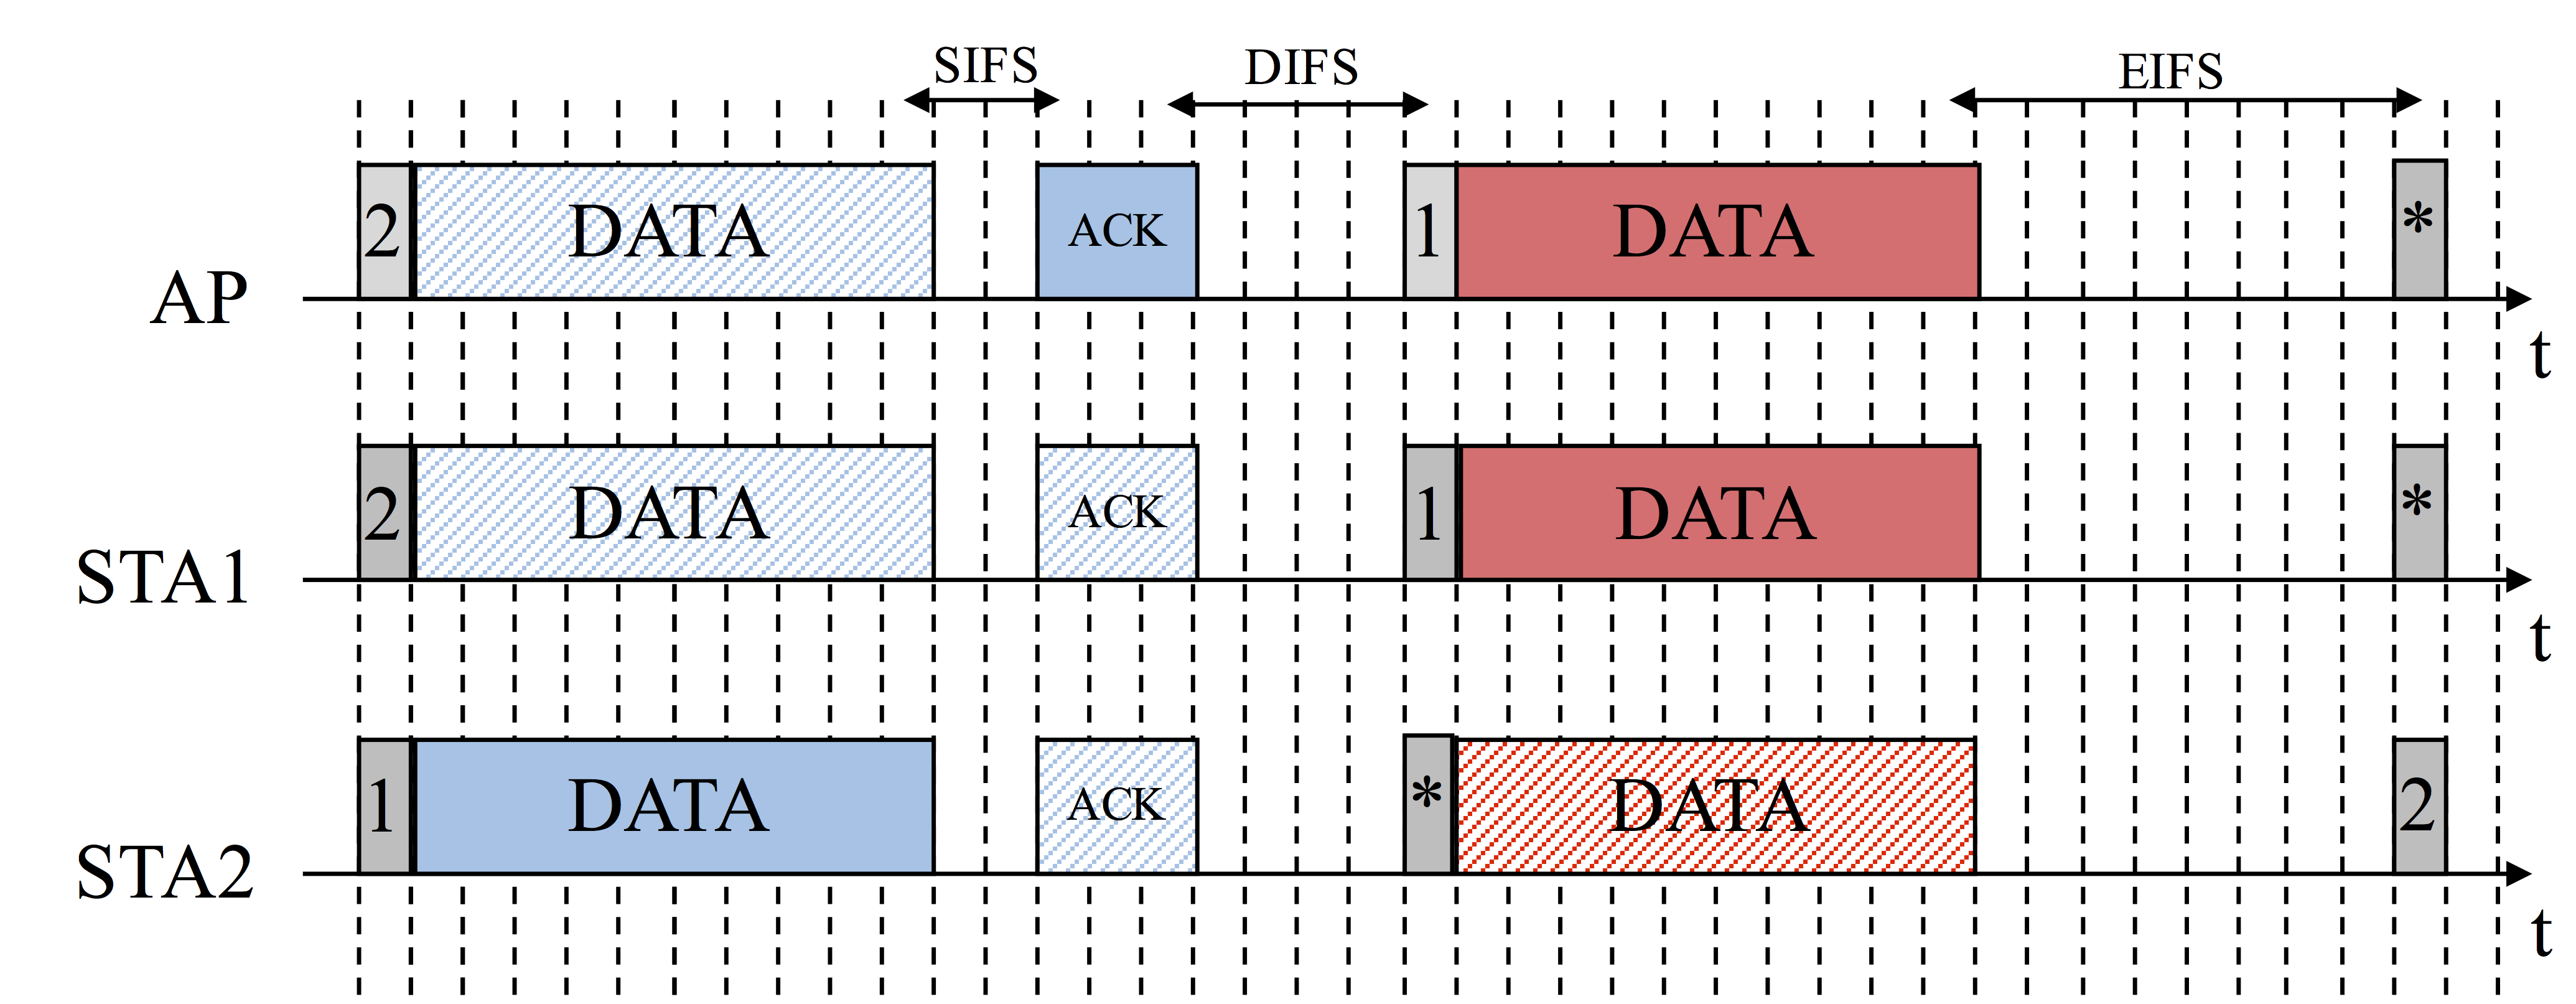
\epsfig{file=images/dcf_operation, width=12cm}
		\caption{DCF operation in a WLAN. STA2 wins the channel access because its initial BO timer is the lowest one. During the packet transmission, STA1 listens the channel busy and stops its BO operation. Once data transmission is finished and the channel has been idle for a DIFS interval, the BO procedure is activated in all the devices that have a packet to be transmitted and sense the channel idle.}
		\label{fig:dcf_operation}
	\end{figure}
	
	At the code level, provided that there are packets in the buffer, a node computes the backoff counter according to its current CW through the \texttt{ComputeBackoff()} function (located at the \texttt{backoff\_methods.h}). Note that the backoff is paused/resumed according to the channel state, and can be checked through the functions \texttt{PauseBackoff()} and \texttt{ResumeBackoff()}, respectively. Moreover, two types of BO are considered, according to the temporal domain. On the one hand, we find \textit{continuous BO}, where time is considered to be continuous, so that collisions by backoff cannot occur. On the other hand, we have \textit{slotted BO}, where the time can be divided in slots, and nodes handle their backoff accordingly. In this case, collisions by backoff can occur, but an important assumption is that nodes are synchronized in some sense (slots are the same for everyone). The type of backoff is indicated by an input parameter.
	
	Regarding the computation of the BO value, note that CW is dynamically adapted on a per-packet basis: CW increases or decreases according to successful/failed transmissions. Given a minimum and a maximum boundaries for CW ($\rm CW_{\rm min}$ and $\rm CW_{\rm max}$, respectively), the reset operation is performed when a successful transmission is carried out. In such situation, the CW is set to $\rm CW_{\rm min}$. Otherwise, when packet losses occur, the CW is increased without exceeding $\rm CW_{\rm max}$. To do so, a counter (namely $\rm CW_{\rm count}$) is maintained and increased one unit each time a packet loss occurs. Then, the CW is computed as $\rm CW = \rm CW_{\rm min} \times 2^{\rm CW_{\rm count}}$. There are two available ways of computing the BO value as a function of the CW: \emph{i)} Uniform: the generated BO is a number between 0 and $\text{CW}-1$, and all the values have the same probability, and \emph{ii)} Exponential: instead of using an uniform distribution, we use an exponential one, so that the generated BO is given by the mean CW value ($\frac{\text{CW}-1}{2}$).

	% RTS/CTS
	\subsubsection{Virtual carrier sensing}
	On top of channel access, we find the data transmission, which in this version of Komondor is done through \textbf{mandatory} Ready-To-Send/Clear-To-Send (RTS/CTS). The RTS/CTS mechanism is implemented in order to minimize the collisions by hidden node. Through RTS/CTS, transmitting nodes attempt to block the channel for the duration of their transmissions. For that, they send RTS packets and wait for confirmation about the clearness of the channel from the receivers' point of view. Through such packet exchange, overlapping nodes must set a virtual carrier sensing during the transmission duration, which allows reducing the collisions by hidden node. The RTS/CTS operation is exemplified in Figure \ref{fig:rts_cts_mechanism}.
	\begin{figure}[h!]
		\centering
		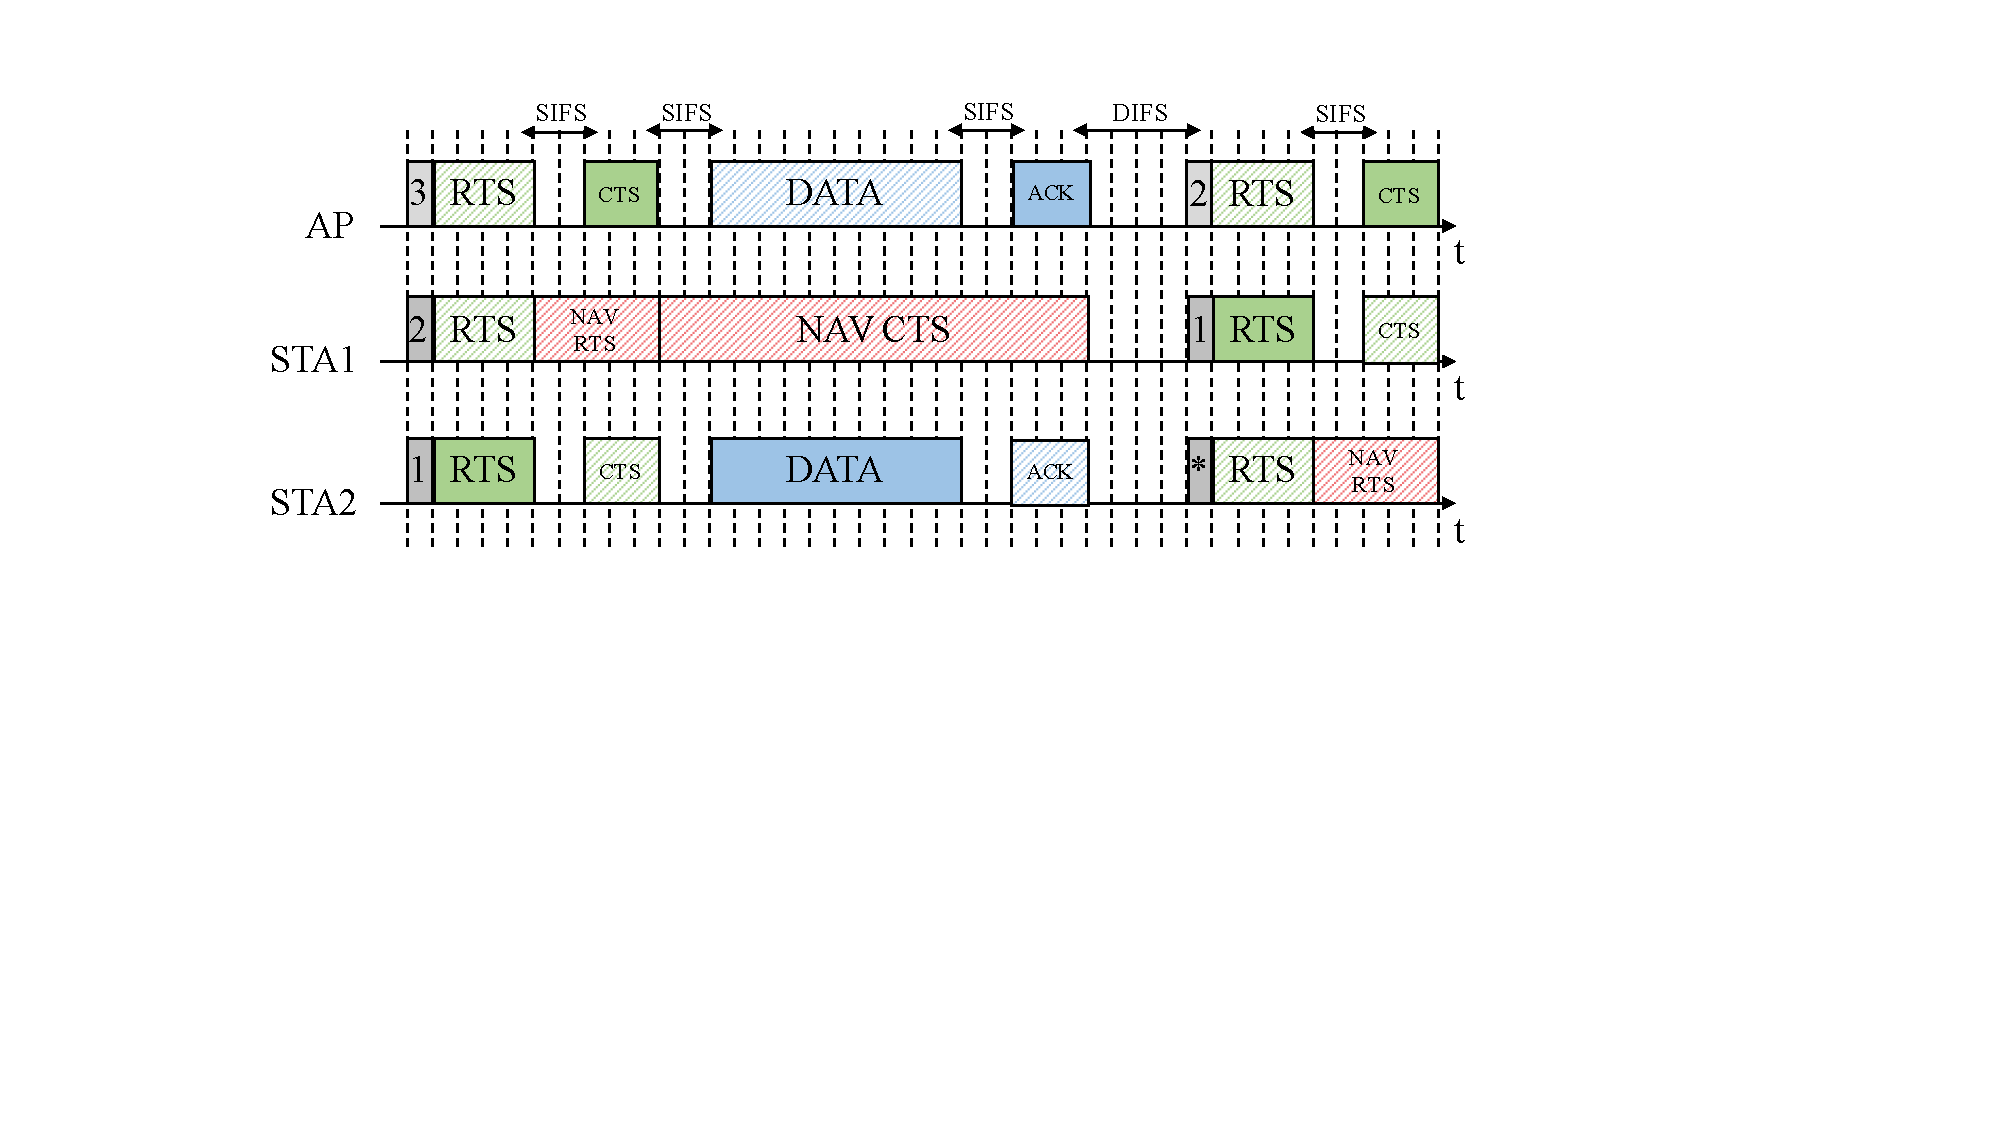
\epsfig{file=images/rts_cts_mechanism.pdf, width=12cm}
		\caption{Example of RTS/CTS implementation. The transmitter (STA2) sends an RTS packet before starting a transmission. The receiver (AP) answers with a CTS as it senses the channel free. The other coexisting devices (STA1) that listen either the RTS and/or the CTS, set their NAV accordingly.}
		\label{fig:rts_cts_mechanism}
	\end{figure}	
	
	In practice, every transmission is initiated with an RTS. Each time a node is able to decode either an RTS or a CTS transmitted to any other recipient, it enters to \texttt{NAV} state. The virtual carrier sensing lasts for the entire transmission (including RTS, CTS, DATA and ACK frames), or until a new transmission updates the NAV timer. In case of being in the \texttt{NAV} state, a given node cannot transmit or receive any kind of data.
	
	% Frames formats
	\subsubsection{Frames formats}
	As previously introduced, the RTS/CTS operation is mandatory in the last version of Komondor. As a result, each data transmission needs to follow the next structure: \emph{1)} Send an RTS frame, \emph{2)} receive a CTS frame, \emph{3)} send the DATA, and \emph{4)} receive an ACK. If any of these frames is lost (refer to Section \ref{section:interference}), the entire transmission is considered to have failed. All the abovementioned frames are defined as in the 11ax amendment and, despite the actual data is not being transmitted in Komondor, the size of each field is respected. The size of each frame is defined in Table \ref{tbl:frame_size}. Note that $L_{\text{SF}}$, $L_{\text{MH}}$ and $L_{\text{TB}}$ are fields that constitute the headers of certain types of frames.
	
	\begin{table}[h]
		\centering
		\begin{tabularx}{\columnwidth}{vbv}
			\toprule
			\textbf{Parameter}     & \textbf{Description}              & \textbf{Value} \\ 
			% PHY and scenario config
			\midrule
			$L_\text{RTS}$        & Length of an RTS packet           & 160 bits       \\ 
			$L_\text{CTS}$        & Length of a CTS packet            & 112 bits       \\ 
			$L_\text{D}$       & Frame size           & 12000 bits     \\ 
			$L_\text{SF}$      & Length of service field       & 16 bits           \\ 
			$L_\text{MH}$      & Length of MAC header     & 320 bits           \\ 
			$L_\text{TB}$      & Length of tail bits     & 18 bits           \\ 
			$L_\text{BACK}$       & Length of a (block) ACK             & 112/432 bits       \\ 
			\bottomrule
		\end{tabularx}
		\caption{Frames size according to the IEEE 802.11ax amendment.}
		\label{tbl:frame_size}
	\end{table}
		
	Apart from standard 11ax frames, packet aggregation is considered, and its utilization can be specified as an input parameter. Roughly, packet aggregation aims at reducing transmission overheads such as headers, SIFS and DIFS intervals or backoff periods. For that, it concatenates $N$ MPDUs to be sent over the same packet transmission, so that it can be acknowledged through a block ACK. Komondor allows to define the number of aggregated packets, which value remains static during the entire simulation.
	\begin{figure}[h!]
		\centering
		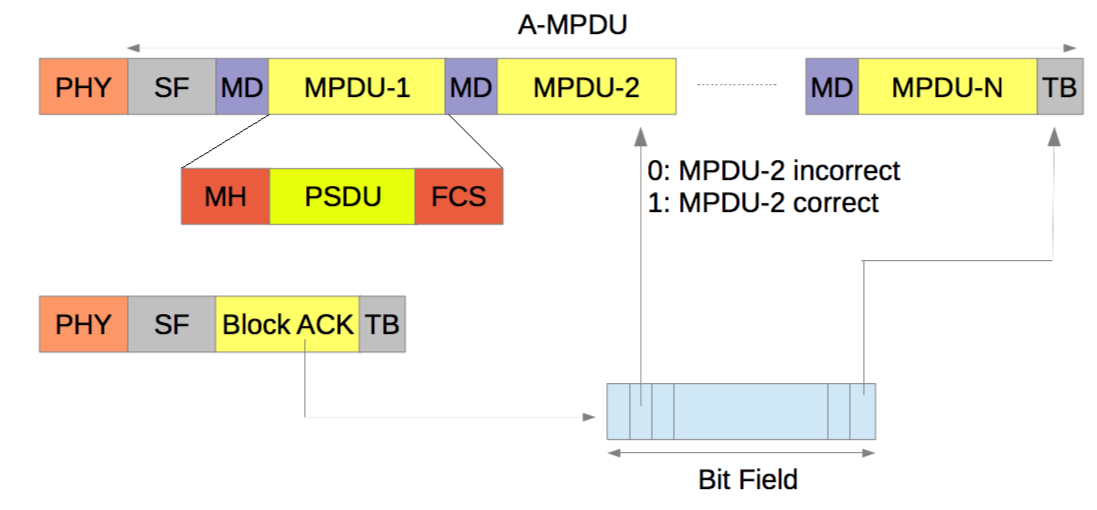
\epsfig{file=images/ampdu, width=10cm}
		\caption{Example of packet aggregation in which N MPDUs are concatenated to be sent during the same packet transmission.}
		\label{fig:ampdu}
	\end{figure}

	In Komondor, every time a transmission is attempted to be initiated, the number of packets to be aggregated is checked, so as the packets available at the buffer. In addition, due to the PPDU duration limitation,\footnote{The maximum PPDU duration defined in the IEEE 802.11 amendment is 5,484 ms.} the number of packets aggregated can be lower than the intended one. In particular, the function \texttt{findMaximumPacketsAggregated()} is responsible to find the maximum number of packets that can be aggregated in a given transmission.
	
	% Transmission times
	\subsubsection{Transmission times}
	The IEEE 802.11ax specification is followed to compute the transmission times. In particular, the time to transmit each data frame (i.e., RTS, CTS, DATA and ACK) is given by:
	
	\begin{equation}
	T_\text{RTS} = T_{\text{PHY-leg}} + \lceil\frac{L_{SF} + L_\text{RTS}}{L_{s,l}}\rceil \cdot \sigma_\text{leg}
	\nonumber
	\end{equation}
	
	\begin{equation}
	T_\text{CTS} = T_{\text{PHY-leg}} + \lceil \frac{ L_{SF} + L_\text{CTS}}{L_{s,l}} \rceil \cdot \sigma_\text{leg}
	\nonumber
	\end{equation}
	
	\begin{equation}
	T_\text{DATA} = T_{\text{HE-SU}} + \lceil \frac{L_{\text{SF}} + L_{\text{MH}} + N_a \cdot L_\text{D}}{L_{s,l}} \rceil \cdot \sigma 
	\nonumber
	\end{equation}
	
	\begin{equation}
	T_{\text{BACK}} = T_{\text{PHY-leg}} + \lceil \frac{L_{\text{SF}} +  L_{\text{BACK}}}{L_{s,l}} \rceil \cdot \sigma_{\text{leg}}
	\nonumber
	\end{equation}
	
	Note that RTS, CTS and ACK (BACK) frames are transmitted in legacy mode. Therefore, the legacy preamble duration, $T_{\text{PHY-leg}}$ is fixed to $20 \mu s$, and the OFDM symbol duration is limited to $4 \mu s$ (OFDM symbol of 24-bits length are used). Regarding the transmission of data, we number of OFDM symbols transmitted depend on the Modulation and Coding Scheme (MCS) used, which at the same time depends on the devices' capabilities. In addition, the duration of an OFDM symbol is now set to $16 \mu s$, since Guard Intervals (GI) of 32 bits are considered. In this case, the preamble duration $T_{\text{HE-SU}} $ is set to $100 \mu s$.
	
	Coming again to the matter of the MCS, the MCS table defined in the IEEE 802.11ax is considered. Komondor assumes that the MCS used between a pair of devices is determined by the SINR at the receiver, so that the maximum allowable MCS is used. The required SINR that corresponds to each MCS is defined in Table \ref{table:sinr_thresholds_mcs}, as well as the granted data rate for each channel width.

	\begin{table}[]
		\centering
		\resizebox{\textwidth}{!}{\begin{tabular}{|c|c|c|c|c|c|c|c|}
				\hline
				\multirow{2}{*}{\textbf{\begin{tabular}[c]{@{}c@{}}MCS \\ index\end{tabular}}} &
				\multirow{2}{*}{\textbf{\begin{tabular}[c]{@{}c@{}}SINR \\ interval (dBm)\end{tabular}}} &
				\multirow{2}{*}{\textbf{\begin{tabular}[c]{@{}c@{}}Modulation\\ type\end{tabular}}} & \multirow{2}{*}{\textbf{\begin{tabular}[c]{@{}c@{}}Coding\\ rate\end{tabular}}} & \multicolumn{4}{c|}{\textbf{Data rate (Mbps)}} \\ \cline{5-8} 
				& &  &  & \textbf{20 MHz} & \textbf{40 MHz} & \textbf{80 MHz} & \textbf{160 MHz} \\ \hline
				0 & {[}-82, -79) & BPSK & 1/2 & 4 & 8 & 17 & 34 \\ \hline
				1 & {[}-79, -77) & QPSK & 1/2 & 16 & 33 & 68 & 136 \\ \hline
				2 & {[}-77, -74) & QPSK & 3/4 & 24 & 49 & 102 & 204 \\ \hline
				3 & {[}-74, -70) & 16-QAM & 1/2 & 33 & 65 & 136 & 272 \\ \hline
				4 & {[}-70, -66) & 16-QAM & 3/4 & 49 & 98 & 204 & 408 \\ \hline
				5 & {[}-66, -65) & 64-QAM & 2/3 & 65 & 130 & 272 & 544 \\ \hline
				6 & {[}-65, -64) & 64-QAM & 3/4 & 73 & 146 & 306 & 613 \\ \hline
				7 & {[}-64, -59) & 64-QAM & 5/6 & 81 & 163 & 340 & 681 \\ \hline
				8 & {[}-59, -57) & 256-QAM & 3/4 & 98 & 195 & 408 & 817 \\ \hline
				9 & {[}-57, -54) & 256-QAM & 5/6 & 108 & 217 & 453 & 907 \\ \hline
				10 & {[}-54, -52) & 1024-QAM & 3/4 & 122 & 244 & 510 & 1021 \\ \hline
				11 & $\geq$ 52 & 1024-QAM & 5/6 & 135 & 271 & 567 & 1143 \\ \hline
		\end{tabular}}
		\caption{Data rates granted per MCS in IEEE 802.11ax. Guard Intervals (GI) of 1600 ns are only considered.}
		\label{table:sinr_thresholds_mcs}	
	\end{table}
	
	So far, link adaptation is not considered\footnote{Future work contemplates the inclusion of Minstrel as a rate adaptation scheme.}. Instead, the MCS to be used between each transmitter-receiver pair is negotiated at the beginning of the first transmission, through the \texttt{RequestMCS()} function. Such a function (which triggers a set of logical events), allows to determine the highest possible modulation between each transmitter-receiver pair. In particular, the SINR is measured at the receiver and the MCS for each set of channels (1, 2, 4 or 8) is provided. It is important to remark that the MCS remains static as long as the scenario does not change (e.g., a new node appears, the transmission power of the transmitted changes, etc.). When something significant changes in the scenario, the \texttt{RequestMCS()} function is triggered again and a new MCS is computed.
	
%%% Upper layer foundations
\subsection{Upper communication layers}

	% Traffic generator
	\subsubsection{Traffic generator}
	\label{section:traffic_generator}
	The traffic generator is intended to simulate the behavior of applications providing data to be transmitted by nodes. To that purpose, we use the \texttt{traffic\_generator.h} class, which is initiated by the main file, according to the data introduced in the ``nodes'' input file. Each transmitter node (only APs are considered transmitters up to this version) is associated with a traffic generator, so that different capabilities can be provided to different WLANs with regards to the generation of application data. Data generation models are further described in Section \ref{section:traffic_modelling}.
	
	\textcolor{red}{[TODO: extend explanation once the traffic generation module has been isolated from node's operation.]}

%%%%%%%%%%%%%%%
%  MODULES
%%%%%%%%%%%%%%%
\section{Modules and Models Available in Komondor}
\label{section:models}
In this Section we present the modules available in Komondor for different communication operations, as well as the current implemented models.

\subsection{Signal Propagation module}
\label{section:propagation}
The signal propagation module can be found at \texttt{power\_channel\_methods.h}, which is located at the \textit{/Komondor/Code/methods} folder. Among several functionalities, this module defines the \texttt{ComputePowerReceived()} function, which computes the power received at a given node, according to the devices' capabilities and the path-loss model. The latter is defined as an input parameter. So far, in order to provide the most representative wireless environments, we implemented the following set of path-loss models, which can be further extended by any developer:
\begin{itemize}
	\item Free Space Path Loss (FSPL): a free-space model is considered, which captures direct line-of-sight and ignores shadowing effects. The experienced loss of power during a transmission that assumes this model is given by:
	\begin{equation}
	\text{FSPL} = 20 \log_{10}(d) + 20 \log_{10}(f) + 20 \log_{10}\Big(\frac{4\pi}{c}\Big) - G_t - G_r,
	\nonumber
	\end{equation}
	where $d$ is the distance between the transmitter and the receiver, $f$ is the frequency used in GHz, $c$ is the light speed in $m/s$, and $G_t$ and $G_r$ are the gains in dB at the transmitter and the receiver, respectively.
	\item Okumura-Hata model \cite{hata1980empirical}: this well-known model was conceived for predicting the path-loss of cellular transmissions in outside urban and rural environments. Since our main concern is related to dense urban areas, let the loss, $L_U$, be given by: 
	\begin{equation}
	\begin{aligned}
	L_U =  &69.55 + 22.16 \log_{10}(f) - 13.82 \log_{10} (h_B) + (44.9 - 6.55 \log_{10}(h_B)) \log_{10}(d) - \\ 
	& 3.2 \log_{10}(11.7554 h_M)^2 - 4.97,
	\end{aligned}
	\nonumber
	\end{equation}
	where $f$ is the center frequency in MHz, $h_B$ is the height of the transmitter antenna, $d$ is the distance between the transmitter and the receiver in meters, and $h_M$ is the height of the receiver's antenna.
	\item Indoor model: this model represents a simple indoor scenario, which is useful to simulate typical scenarios such as flats, schools or restaurants. According to this model, the loss, $L_{indoor}$, experienced during a transmission is:		
	\begin{equation}
	L_{indoor} = \text{PL}_f + 10 \alpha \log_{10}(d) + h_s + \Big(\frac{d}{f_w}\Big) h_o,
	\nonumber
	\end{equation}
	where $\text{PL}_f$ is the path-loss factor, $\alpha$ is a constant that depends on the propagation model, $d$ is the distance in meters between the transmitter and the receiver, $h_s$ is the shadowing factor, $f_w$ is the frequency of walls, and $h_o$ is the obstacles factor.
	
	Furthermore, a variation of this path-loss model is provided, in order to introduce random variables that determine the shadowing and obstacles effects in the power losses.
	\item Residential path-loss model IEEE 802.11ax: such model is included in the 11ax amendment, and captures the path-loss effects of a typical apartments building. The loss, $L_{indoor-ax}$, experienced during a transmission is given by:
	\begin{equation}
	\begin{aligned}
	L_{indoor-ax} = &40.05 + 20 \log_{10}\Big(\frac{f_c}{2.4}\Big) + 20 \log_{10}(\min(d,5)) + (d>5)  35 \log_{10}\Big(\frac{d}{5}\Big) + \\
	&18.3 F^{\frac{F+2}{F+1}-0.46} + 5 W,
	\end{aligned}
	\nonumber
	\end{equation}
	
	where $f_c$ is the frequency in GHz, $d$ is the distance between the transmitter and the receiver, $F$ is the number of floors traversed, and $W$ is number of walls traversed in the x-direction plus the number of walls traversed in the y-direction
\end{itemize}	

On top of the path-loss model, we also defined the possibility of using different adjacent channel interference models, which determine the amount of power leaked into adjacent channels. The fact of using non-overlapping channels entails more aggressive interactions given that devices in other channels also contribute to the sensed interference in a given receiver. An example of channels overlapping is shown in Figure \ref{fig:cochannel_interference}.
\begin{figure}[h!]
	\centering
	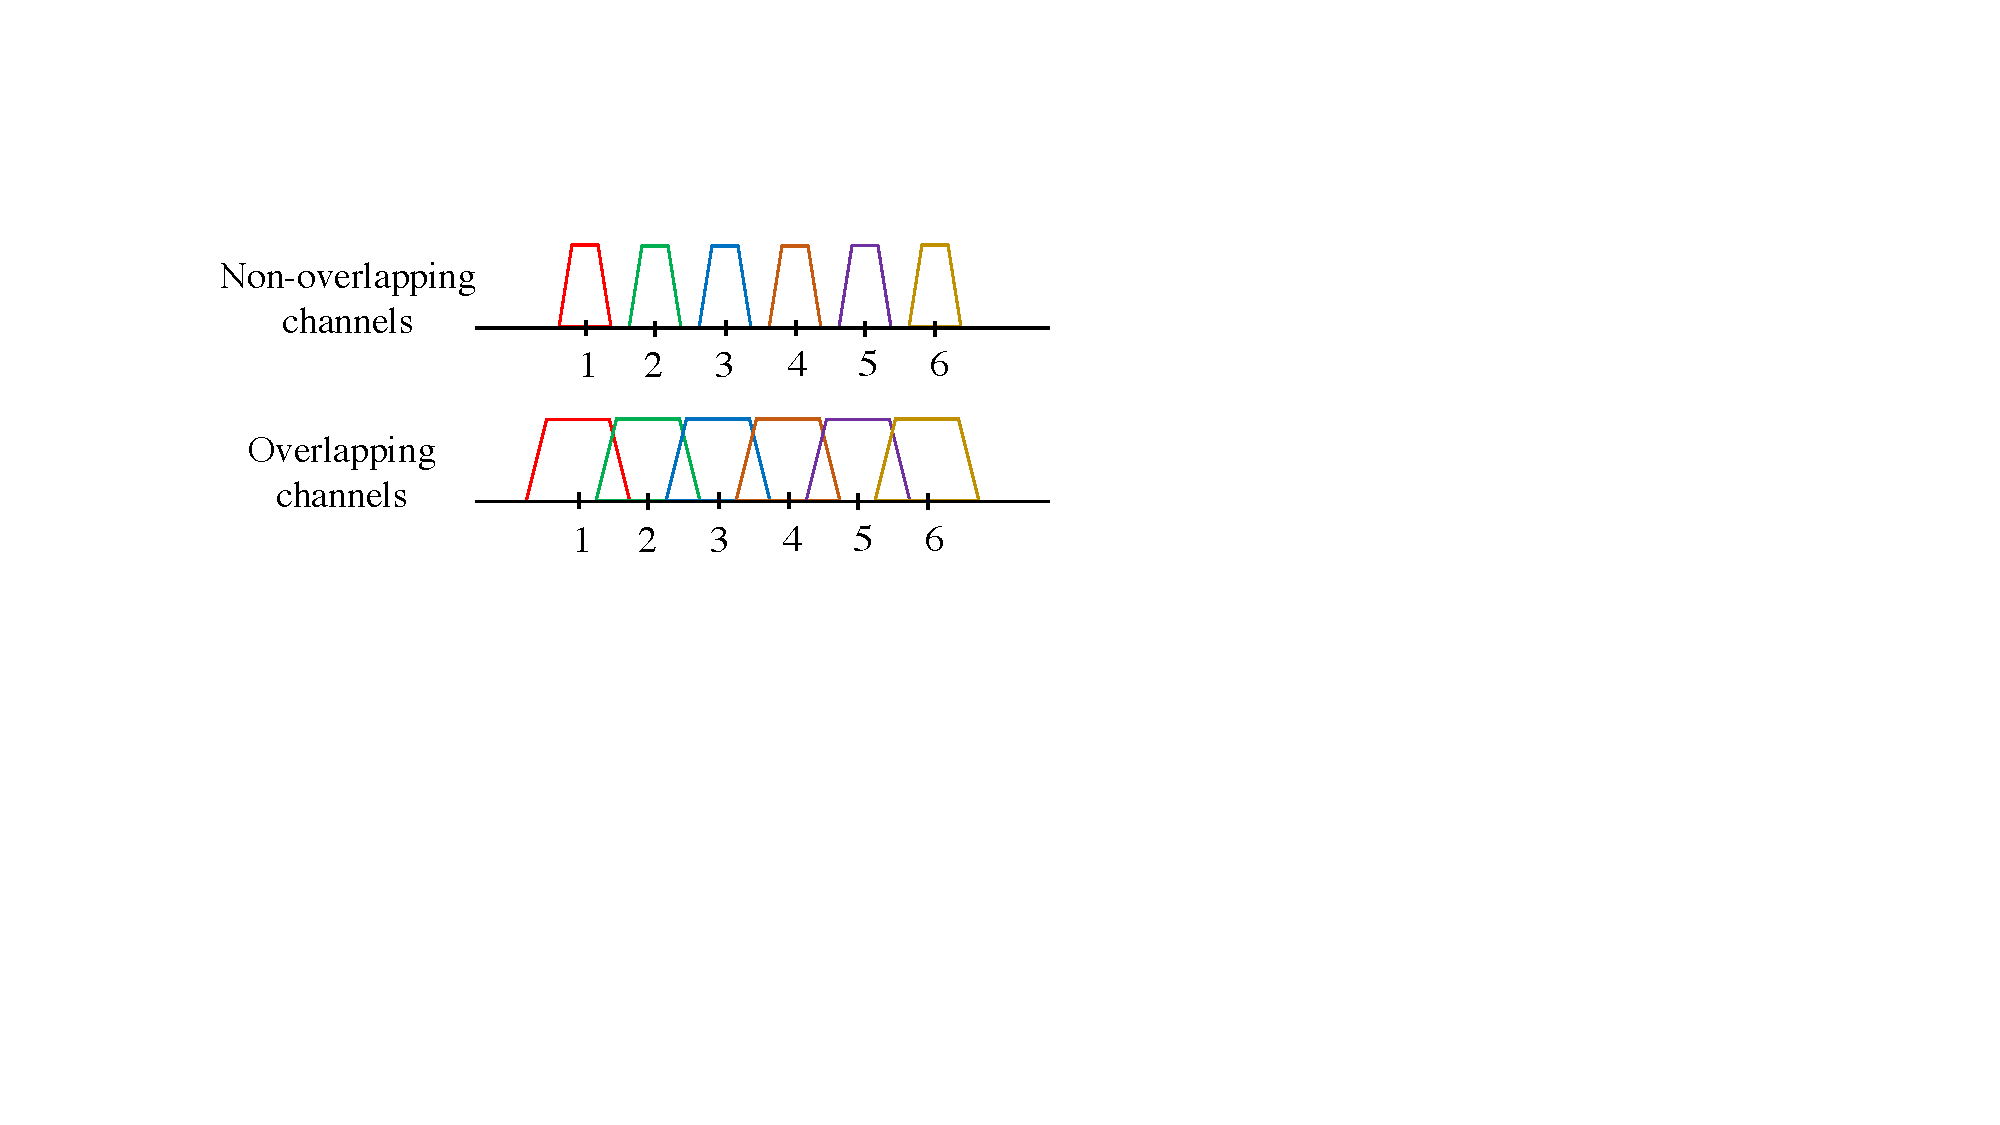
\epsfig{file=images/cochannel_interference.pdf, width=9cm}
	\caption{Channel models with and without ACI}
	\label{fig:cochannel_interference}
\end{figure}	

In particular, Komondor includes the following ACI models:		
\begin{itemize}
	\item \textbf{No interference}: no power is leaked to adjacent channels.
	\item \textbf{Total interference}: power from other channels is leaked, so that a 20 dB decrease is noticed for each channel distance. For instance, the power that channel 1 leaks into channel 3 is the actual power in channel 1 minus 40 dBr. 
	\item \textbf{Limited interference}: in this case, only immediate adjacent channels leak power to the target one, so that a 20 dB decrease is noticed from consecutive channels.
\end{itemize}

Recall from Section \ref{section:phy} that the power sensed at a given receiver is assumed to be the same during the entire transmission. This relaxation allows us to easily determine whenever the channel of interest is busy or not. A direct implication of it affects to path-loss models used, as well as some of them assume random variations of the medium, preventing to obtain the same result with different power received calculations (so far, power received is added and subtracted when the node accesses and leaves the channel, respectively). Thus, for each node, Komondor stores the incoming power of a given transmission when it begins and subtracts the power when it is over. 

\subsection{Traffic generation module}
\label{section:traffic_modelling}
The traffic generator has been previously defined in Section \ref{section:traffic_generator}. Here we describe the traffic models already provided, which are included in the \texttt{traffic\_generation\_methods.h}. In particular, we have considered three different models:
\begin{itemize}
	\item \textbf{Full buffer}: transmitters are in a permanent saturation regime, so that they always have packets to be sent.
	\item \textbf{Poisson}: packets are generated according to a Poisson distribution process, so that the average time between packets is determined by the packet generation rate $\lambda$, and which is given by $\Delta_{\rm p} = \frac{1}{\lambda}$.
	\item \textbf{Deterministic}: packets are generated at fixed time intervals given by the packet generation rate, $\Delta_{\rm d} = 1/\lambda$.
\end{itemize}

Figure \ref{fig:traffic_models} illustrates the aforementioned traffic models. 
\begin{figure}[h!]
	\centering
	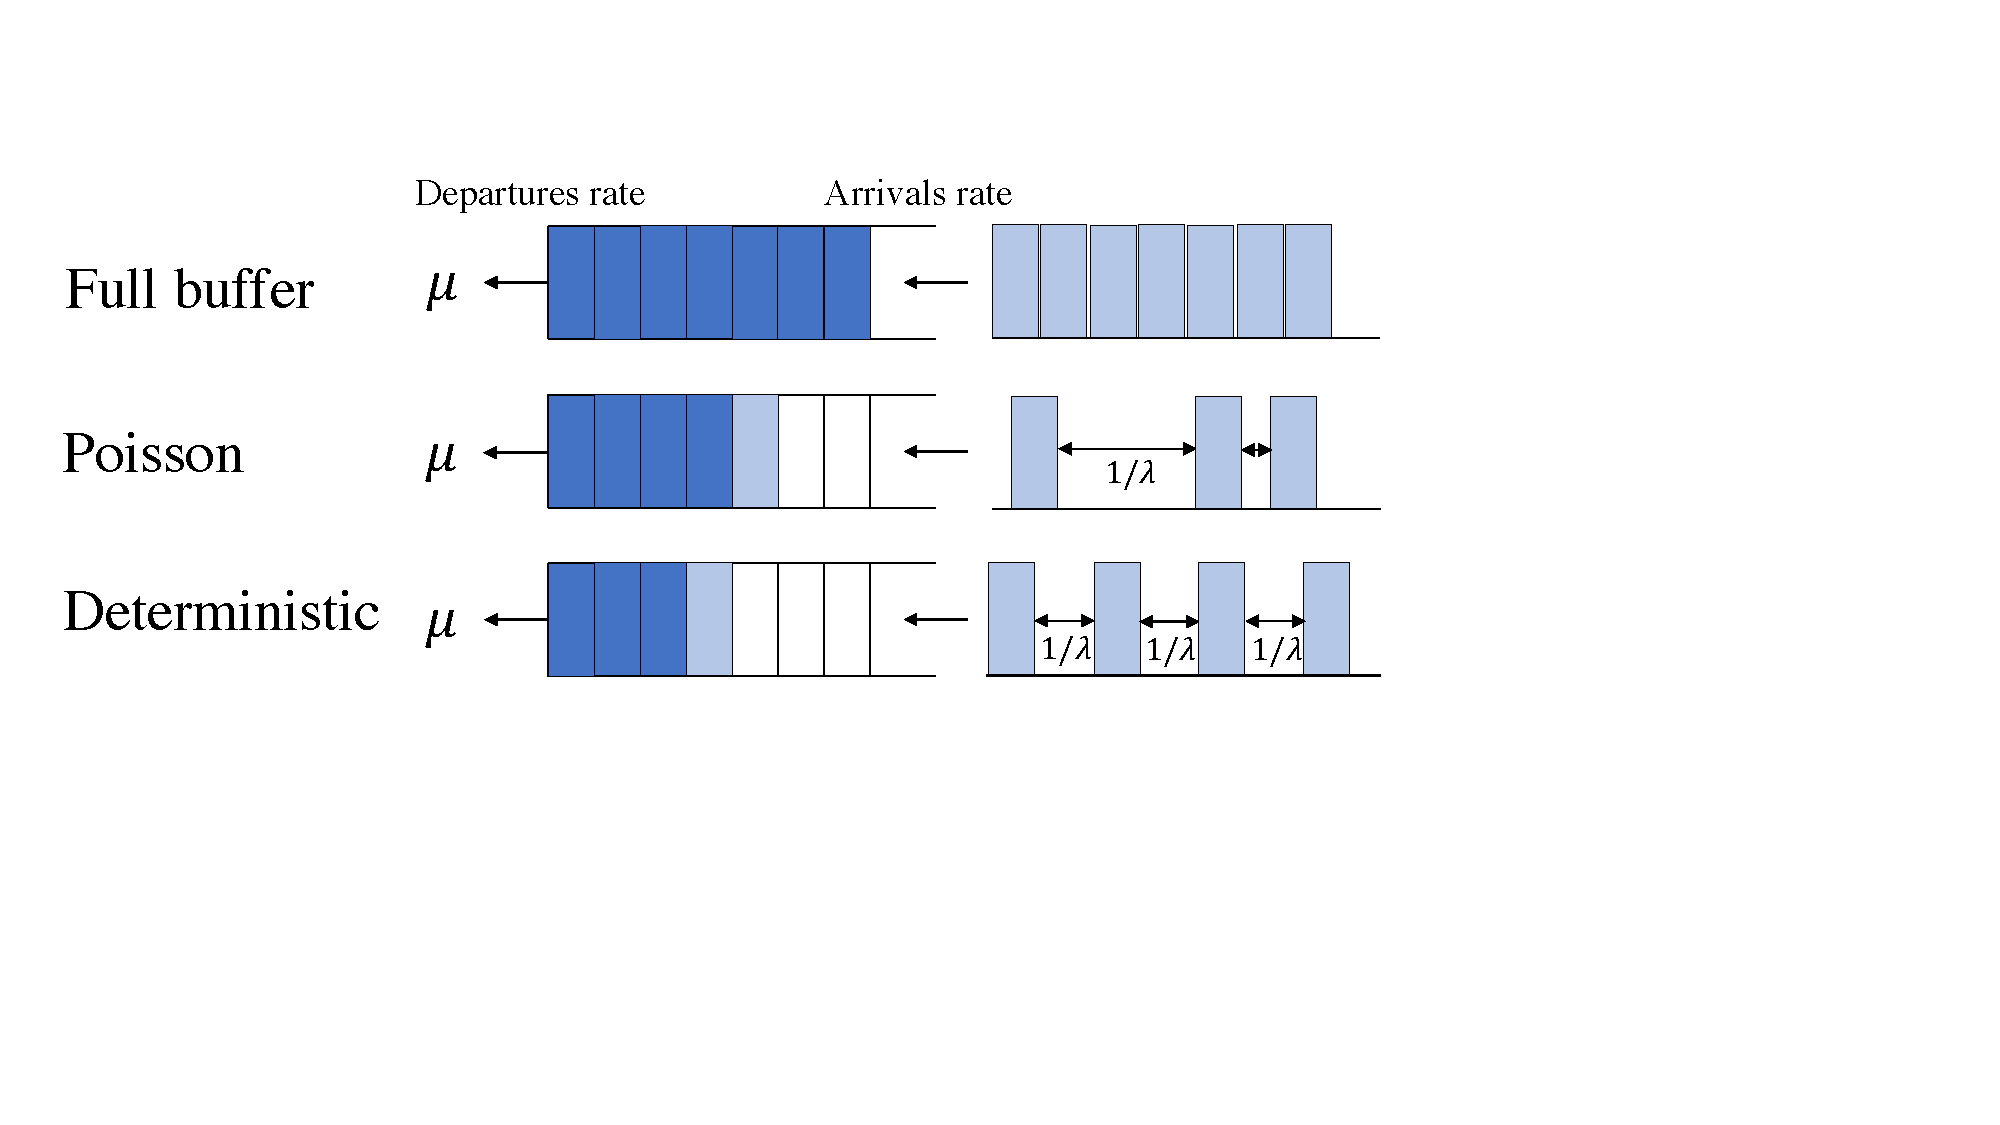
\epsfig{file=images/traffic_models.pdf, width=9cm}
	\caption{Traffic models used in Komondor}
	\label{fig:traffic_models}
\end{figure}	

\subsection{Backoff generation module}
As shown in Section \ref{section:mac}, two different backoff modules are considered, namely slotted and continuous backoff. However, we also defined two different ways of computing the value backoff, independently of whether it is embedded into slots or not.
\begin{itemize}
	\item Deterministic: the backoff value is generated uniformly at random between 0 and CW - 1.
	\item Exponential: the backoff value is generated following an exponential distribution centered in $\lambda$, where $\lambda = 1/\text{E[BO]}$
\end{itemize}

\subsection{Dynamic Channel Bonding module}
Dynamic channel bonding (DCB) is one of the most promising techniques to enhance spectral efficiency in IEEE 802.11ax WLANs, since it aims to make the most of the medium by transmitting data over several contiguous basic channels. For that, different DCB policies are implemented in Komondor, which can be interchangeably applied by the simulated WLANs. To perform DCB, one may explicitly define the available range of basic channels for each WLAN. Then, the following policies have been defined in \texttt{GetTxChannelsByChannelBonding()}:
\begin{itemize}
	\item \textbf{Only Primary (OP)}: the legacy operation is performed, so that only the primary channel is attempted to be accessed. This policy is also known as single-channel.
	\item \textbf{Static Channel Bonding (SCB)}: carrier sensing is performed at the primary channel. However, when attempting to transmit, all the channels within the CB range must be clear. Otherwise, a new backoff is computed.
	\item \textbf{Always-max (AM)}:\footnote{Some papers in the literature use the terms DCB and AM indistinctly. In this document we notate AM as an special case of DCB.} picks the widest possible channel found free for transmitting. Note that, in order to include secondary basic channels for transmitting, a WLAN must listen them free during at least a PIFS period before the backoff counter terminates as shown in Figure \ref{fig:dcb_dcf}.
	\begin{figure}
		\centering
		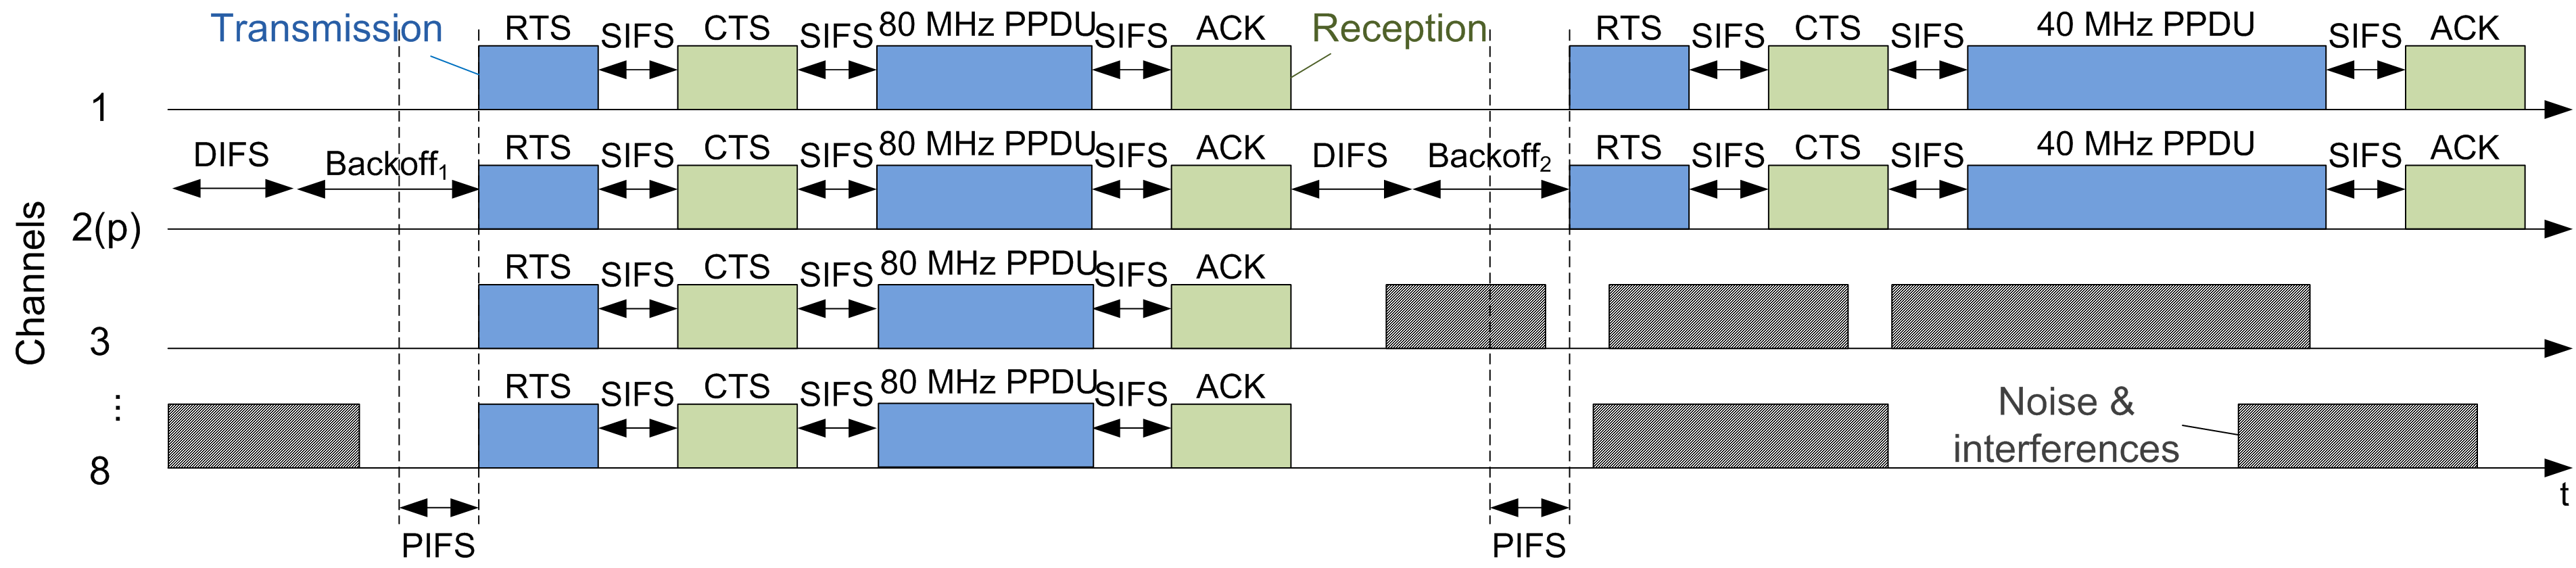
\includegraphics[width=0.95\textwidth]{images/dcb_dcf.png}
		\caption{CSMA/CA temporal evolution of a node operating under AM and the IEEE 802.11ax channelization scheme.}
		\label{fig:dcb_dcf}
	\end{figure}
	\item \textbf{Probabilistic uniform (PU)}: picks with same probability any of the possible channels found free inside the allocated channel.
	
\end{itemize}

For the sake of illustration, let us consider the example shown in Figure \ref{fig:dcb_dcf}, where the evolution of a node implementing AM is presented. Regarding the rest of DCB policies, \textit{i}) OP would just pick channel 2 after both backoff terminations, \textit{ii}) SCB would only transmit after the first backoff termination as part of the rest of basic channels is busy after the second one, and \textit{iii}) PU would transmit on channels $\{2\}, \{1,2\}, \{1,2,3,4\}$ or $\{1,2,...,8\}$ with same probability (1/4) at the first backoff termination, and on channels $\{2\}$ or $\{1,2\}$ with probability 1/2 at the end of the second one. An schematic flowchart of the DCB policy operation is shown in Figure \ref{fig:cb_policy_flowchart}.

\begin{figure}[h]
	\centering
	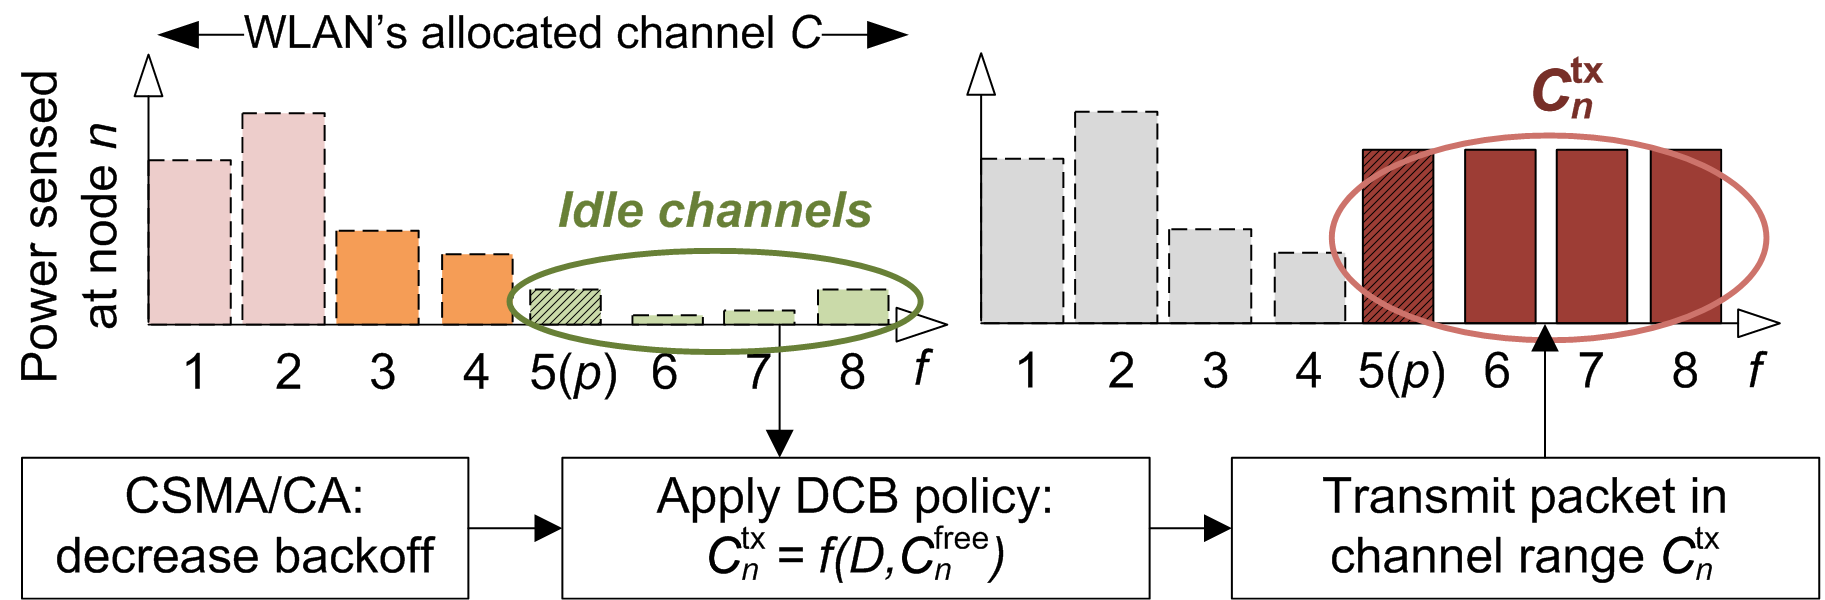
\includegraphics[width=0.64\textwidth]{images/cb_policy_flowchart.png}
	\caption{Flowchart of the transmission channel selection. In this example channel 5 is the primary channel and AM is applied.}    
	\label{fig:cb_policy_flowchart}
\end{figure}

%%%%%%%%%%%%%%%
% AGENTS
%%%%%%%%%%%%%%%
\section{Agents in Komondor}
\label{section:agents}
The Komondor simulator includes a set of modules that allow simulating the operation of WLANs with embedded agents. So far, for the release v.2.0 (\textcolor{red}{TODO: clarify this}), decentralized agents are fully implemented. Note, as well, that the communication infrastructure for enabling both distributed and centralized is available. However, Komondor is not yet ready to support these operational modes. Intensive work about a Machine Learning (ML) architecture is currently in progress, where all the learning modes are being defined in the context of Komondor. 

Komondor incorporates agent entities (\texttt{agent.h} class), which are associated to nodes and are responsible of monitoring their performance and performing recommendations for certain configurable parameters. Accordingly, Komondor seeks to simulate an agent-based infrastructure where APs contain the necessary intelligence to learn in a decentralized manner.\footnote{Decentralized learning frames a situation in which WLANs are able to learn based on their own performance information (further information can be found in \cite{wilhelmi2017implications, wilhelmi2017collaborative, wilhelmi2018potential}).} Note, as well, that a single agent can be associated to a given WLAN, and the communication is held only with the AP.

The agent entity is therefore responsible of the following functionalities:
\begin{itemize}
	\item Make queries to the agent to retrieve information regarding its current performance (e.g., packets sent/lost, delay, etc.) and configuration (e.g., transmission power, number of associated STAs, etc.).
	\item Process the information obtained from the AP and execute a given learning-based operation.
	\item Generate a new configuration to be suggested to the AP.
\end{itemize} 

Figure \ref{fig:agents_komondor} illustrates the operations held by an AP and its embedded agent during the learning procedure. Both entities communicate each other through a set of inports/outports. Note, as well, that such a communication occurs at certain intervals that can be indicated by the input. In addition, delays can be added to simulate different architectural limitations (e.g., hardware delay). 

\begin{figure}[h]
	\centering
	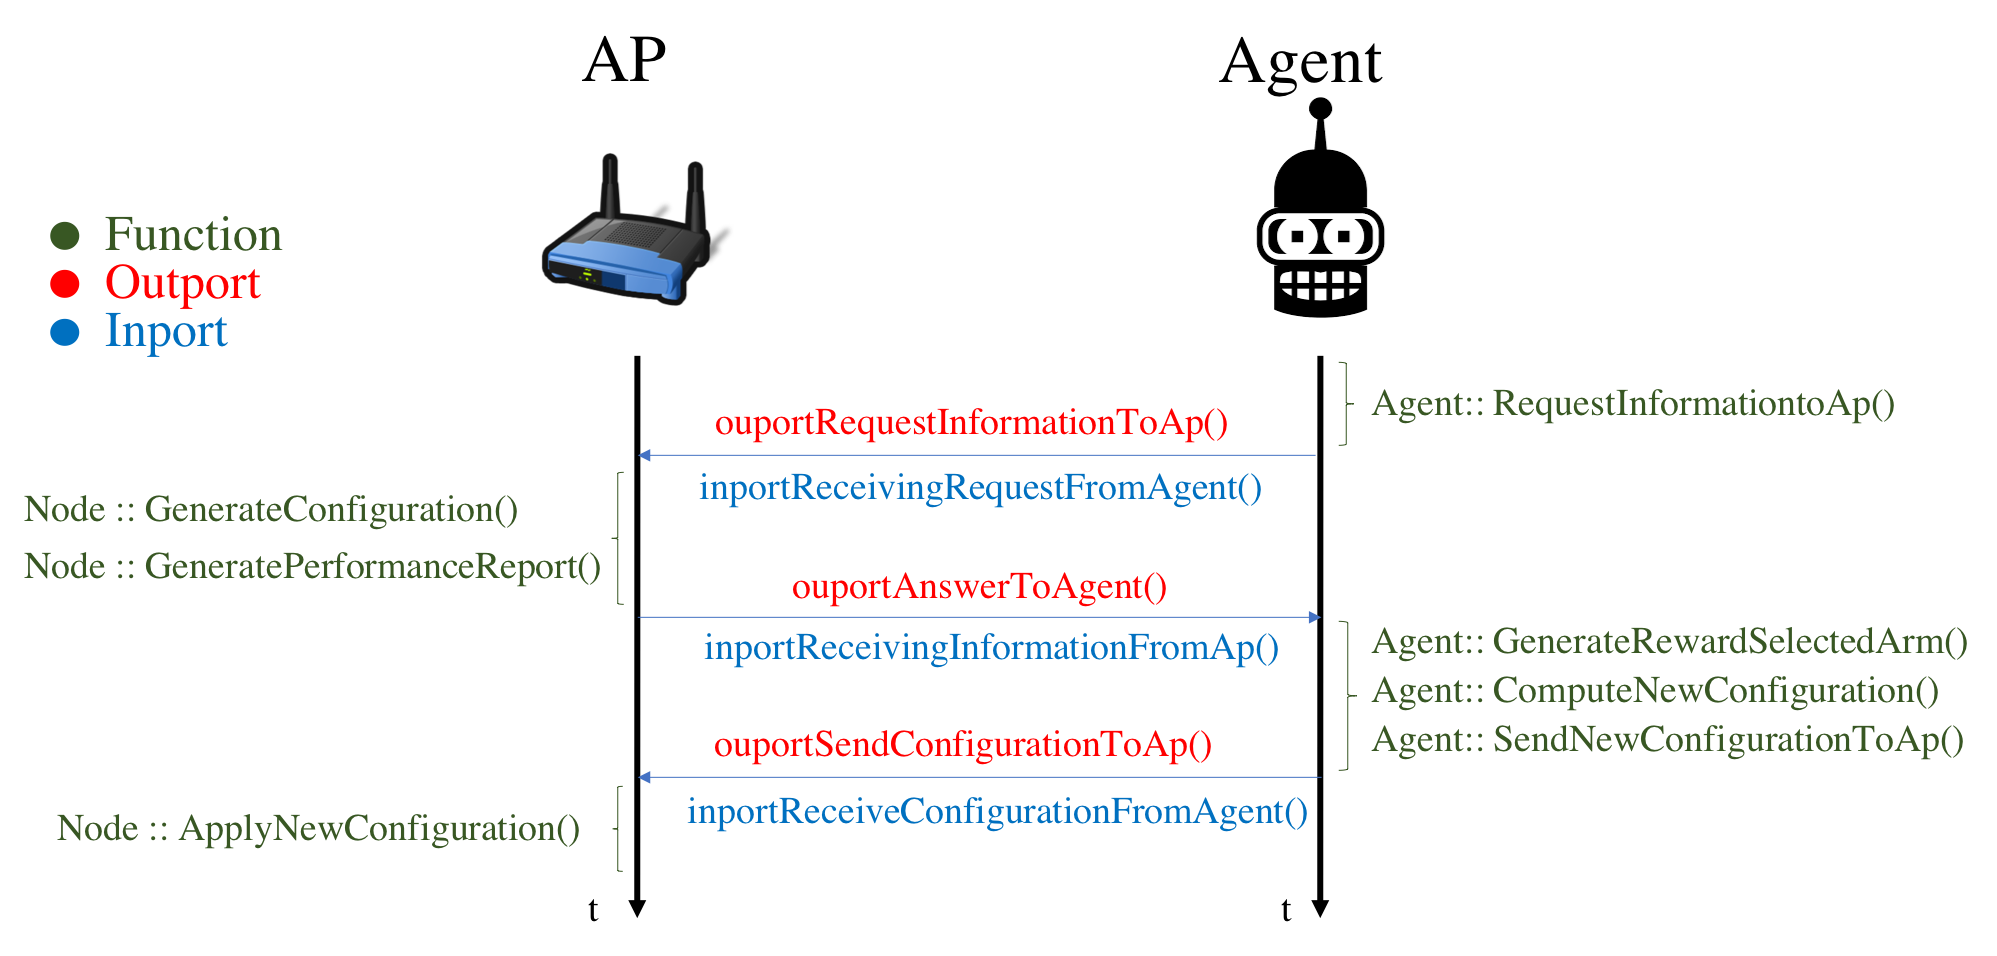
\includegraphics[width=\textwidth]{images/agents_komondor.png}
	\caption{AP-agent communication-based operation in Komondor.}    
	\label{fig:agents_komondor}
\end{figure}

It is important to note that \texttt{agent.h} is responsible of orchestrating the learning operation through the communication with the AP. The learning mechanisms are independent modules that are used by the agent and which must be placed at the \textit{Komondor/main/learning\_modules} folder. So far, we provided the \texttt{multi\_armed\_bandits.h} class, which includes the necessary functions to apply the Multi-Armed Bandits framework \cite{auer2002finite}. Such a class is responsible of handling the environment through which MAB-based strategies can be applied. In other words, it processes the information provided by the agent (performance and configuration) to generate the necessary data structures that allow implementing certain action-selection strategies. Once the data is prepared for the MAB operation, the new configuration is obtained according to the chosen action-selection strategy. For code modularization purposes, we provided a subfolder (i.e., \textit{Komondor/main/learning\_modules/action\_selection\_strategies}) containing different action-selection strategies such as $\varepsilon$-greedy \cite{sutton1998reinforcement} or Thompson sampling \cite{thompson1933likelihood}.

The project has been therefore conceived so that any interested researcher can easily implement a given learning mechanism (either online or offline), thus making use of a flexible infrastructure.

%%%%%%%%%%%%%%%
% TUTORIAL
%%%%%%%%%%%%%%%
\section{Development Notes}
\label{section:tutorial_and_development_notes}
Here we provide some clarifications regarding code implementation, wit the aim to facilitate the Komondor's usage and manipulation to developers that may be interested.
	
	% Considerations
	\subsection{Main considerations}
	\label{section:development_considerations}
	% TODO: Extend this part.
	Some technical information regarding code development is worth to be mentioned to properly understand how to use and modify the Komondor simulator. So far, the main considerations to be taken into account are:		
	\begin{itemize}
	\item \textbf{Power and CCA}: power variables are stored in pW (pico watts) in order to be able to operate power magnitudes without loosing resolution\footnote{For instance., the sum of two signals of power values -85 dBm (3.162 pW) and -90 dBm (1 pW), respectively, is -83.803 dBm (4.162 pW).}. However, values are presented to the user in dBm.		
	W (-30)  - mW (0)  - uW (+30) - nW (+60) - pW (+90)\\
	$P_{\text{pw}} = 10^{\frac{P_{\text{dBm}} + 90}{10}}$
	\end{itemize}

	% Miscellany
	\subsection{Miscellaneous}
	\label{section:development_miscellany}
	% TODO: Extend this part.
	\begin{itemize}
	\item \textbf{Transmitting capability}: we have added a flag to each node that determines if it is able to transmit (1) or not (0), so that we can decide if the node is only listening or both transmitting and listening.
	\item \textbf{Progress bar}: the Komondor simulation progress bar is displayed through a \textit{printf()} command called by any node with \textit{node\_id} set to 0. If no node has \textit{node\_id} set to 0, the progress bar is not displayed.
	\end{itemize}
	
%%%%%%%%%%%%%%%
% CONCLUSIONS
%%%%%%%%%%%%%%%
\section{Conclusions Future Development Notes}
\label{section:conclusions}

In this document we provided an overview of the first version of the Komondor simulator, which aims to reproduce the basic operation of IEEE 802.11ax WLANs in addition to allow the utilization of intelligent systems. We introduced the system model considered when building the simulator, as well as the main MAC features implemented. Additionally, due to the open source nature of this project, we provided basic information of interest for developers that are expected to use or even modify this HD WLANs simulator.

This project is expected to move forward for including of novel mechanisms such as OFDMA, MU-MIMO, TPC or  CST adjustment. In addition, intelligent agents are expected to be included for making operations such as Dynamic CB (DCB).

%%% BIBLIOGRAPHY
\bibliographystyle{unsrt}
\bibliography{bib}

\end{document}